\setstretch{1.4}
\sectiontitle{6}{2D Path following}
\lhead{2D Path following} % section header
This final section describes how 2D path following was achieved for the ribbon robot. It begins with an analysis of some relevant literature, it then describes the kinematic model designed for the system and the control systems final design, which combines all the components described in previous chapters as well as a closed-loop pitch control and Integral-Line-Of-Sight (ILOS) guidance system. The implementation of these two last components is then explained as well as the device-specific adaptation method implemented due to differences in device dynamics. This all finally enables real-time following of preset paths through the brain phantom, the results of which are presented and discussed. The final subchapter then discusses some possible future developments.

\lhead{2D Path following - Background} % section header
\subsection{Background}
\subsubsection{Kinematic Modeling of Similar Devices}
Devices with kinematic similarities to the tendon-driven ribbon-shaped device primarily include steerable needles, concentric tube robots, and tendon-drive continuum robots. Each of these devices rely on structural flexibility and and actuation mechanism that creates a curvature or deformation that allows for navigating through soft biological tissues. However none of their models are directly applicable.
\begin{figure} [H]
    \centering
    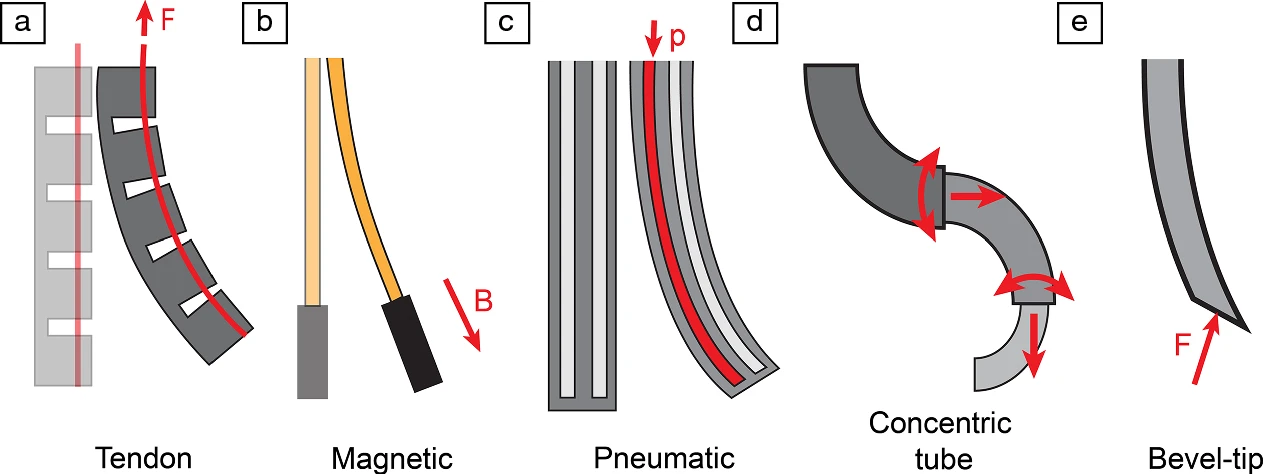
\includegraphics[width=0.9\linewidth]{images/steerableNeedles/actuations.png}
    \caption{Illustration of main actuation and steering mechanisms of small-scale robotic devices developed for brain interventions. Robotic devices can be navigated using (a) tendon-driven mechanisms, (b) magnetic forces and torques, (c) pneumatic systems,  (d) concentric tubes, and (e) slender features with beveled tips. \cite{noseda_small-scale_2024}}
    \label{fig:actuations}
\end{figure}

\paragraph*{Magnetic, Pneumatic and Concentric Tube robots}
Most steerable robotic devices are actuated in a fundamentally different manner to the tendon driven ribbon device and must therefore also be steered in a very different way. Magnetic actuation typically relies on external magnetic fields interacting with embedded magnets in the device \cite{petruska_magnetic_2016} \cite{pancaldi_flow_2020}. Pneumatic systems induce curvature by inflating internal chambers which results in a deformation along the entire device  \cite{gopesh_soft_2021}, \cite{luo_novel_2023}. Concentric tube robots utilize nested tubes with pre-defined curvatures actuated through relative rotation and translation \cite{dupont_continuum_2022}, \cite{alfalahi_concentric_2020}. Consequently all of these devices kinematics models are not directly transferable to tendon-driven ribbon-shaped devices.

\paragraph*{Traditional tendon-driven continuum robots}
Traditional tendon-driven continuum robots differ significantly to the device used here in their modeling despite their similar actuation. This because they deform continuously along their entire length of a segment under actuation forces. While in the ribbon device here it deforms primarily at the distal tip due to the interaction between the backbone and the surrounding brain tissue. Therefore existing continuum robot kinematic models \cite{chitalia_design_2020} \cite{kato_tendon-driven_2016}, which assume distributed deformation, cannot be directly applied.

\paragraph*{Steerable Needles}
The device that is by far closest in its steering mechanism are steerable needles. Primarily since steerable needles utilize a deformation at only the tip in order to induce curvature during insertion which can be achieved in several distinct ways \cite{van_de_berg_design_2015}. This leads to nonholonomic kinematics , meaning the needle's orientation and position are coupled in a way that constrains its possible instantaneous directions of movement i.e. it cannot more laterally without insertion \cite{webster_nonholonomic_2006}. The mechanics have been thoroughly studied for these devices leading to the development of both kinematic and dynamic models \cite{misra_mechanics_2010}. Although steerable needles typically achieve directional control be rotating the bevel tip or moving segment of the tip as in Secoli et al's work \cite{secoli_adaptive_2016} \cite{secoli_closed-loop_2013}, their steering is still a highly relevant foundation for kinematic models for the tendon-driven ribbon-shaped device.
\newline \newline 
An effective 2D model was developed by Young Ko et al in \cite{ko_two-dimensional_2010}. The steerable probe is modeled as a planar nonholonomic system, where the curvature at the tip determines the trajectory insertion. This curvature is treated as an input to a unicycle-like kinematic model where the evolution of the probe's pose is governed by its insertion velocity and current curvature.
\begin{figure} [H]
    \centering
    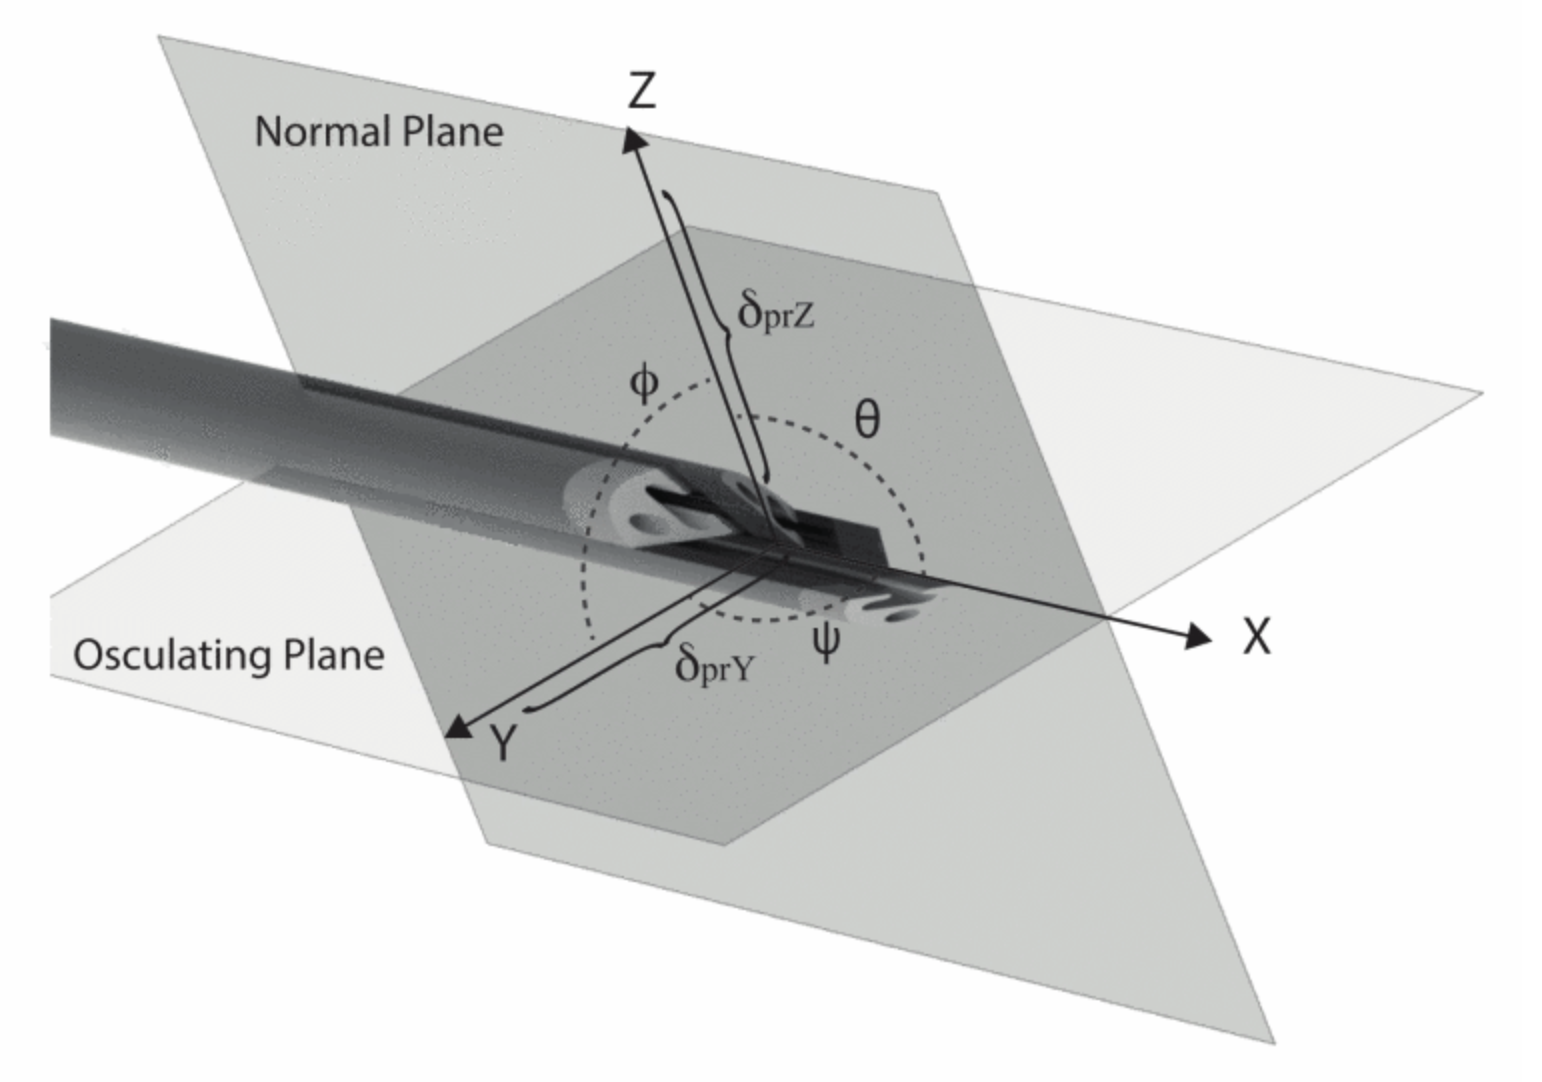
\includegraphics[width=0.7\linewidth]{images/steerableNeedles/needlefig.png}
    \caption{Four part Steerable needle developed by Secoli et al \cite{secoli_closed-loop_2013}}
    \label{fig:fourpartneedle}
\end{figure}
Later Secoli and Rodriguez y Baena developed a 3D version for the same 4-part steerable needle (seen in figure \ref{fig:fourpartneedle}) inspired by underactuated underwater vehicles. The needle's motion is governed by nonholonomic constraints, with insertion along the x-axis and tip steering controlled by programmable offsets between interlocked needle segments. The model defines the needle's orientation using Euler angles (roll, pitch, yaw), with angular velocities about the pitch and yaw axes proportional to the segment offsets. This results in a non-linear, driftless kinematic system, which they then convert into chained form coordinates for closed-loop feedback control.

\begin{figure}
    \centering
    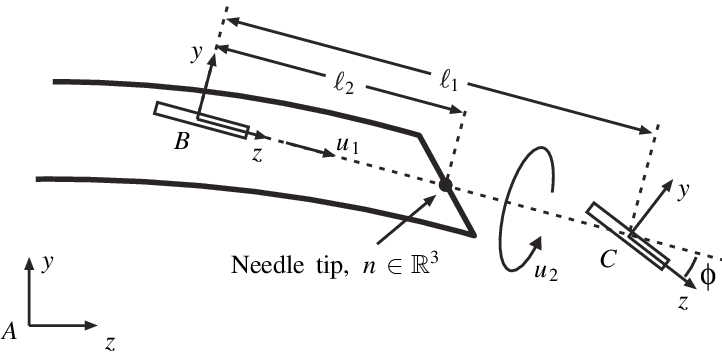
\includegraphics[width=0.7\linewidth]{images/steerableNeedles/Configuration-of-a-bevel-tip-needle-during-steering-showing-the-front-and-back-wheels.png}
    \caption{Configuration of a bevel tipped needle during steering showing the front and back "wheels" \cite{webster_nonholonomic_2006}}
    \label{fig:bicycle}
\end{figure}
A more complex strategy for modeling needle steering is the  model introduced by Webster et al. \cite{webster_nonholonomic_2006}, which treats needle insertion as a constrained control problem similar to a bicycle instead of a unicycle. In bevel-tip needles, the asymmetry at the tip induces lateral forces during insertion naturally creating a curved trajectory where orientation and position are interdependent \cite{misra_mechanics_2010}. For a fixed needle shaft rotation, the model is similar to that of a bicycle with a front wheel angle and a back wheel angle that corresponds to the angle a certain distance from the tip of the needle \cite{webster_nonholonomic_2006} as is shown in figure \ref{fig:bicycle}.
\newline \newline
Fallahi et al. extended this model for soft tissue and created a model that accounts for non-constant curvature paths for the needle tip. Since for a tissue that is not stiff relative to the needle, the tissue deformation caused by needle insertion deviates the needle tip position. This model is obtained by replacing the bicycle wheels with omnidirectional wheels that move in two orthogonal direction independently. Such wheels can move sideways, providing a means for modeling the deviations of the needle tip from a constant curvature path. \cite{fallahi_extended_2015}


\subsubsection{Path Following Definition}
Path following is a  motion control scenario where a “vessel” has to follow a predefined path without any time constraints \cite{caharija_integral_2016}. It thereby differs to trajectory tracking since the path is not parameterized by time, but rather by another useful parameter \cite{hung_review_2023}, such as path length. 

This distinction is important since in the application to brain surgery spatial control is a lot more critical than timing. Also since the system can make smoother corrections and prioritize accuracy over speed when there are no strict time requirements. Path following also allows smoother convergence to the path and can reduce actuator actuator activity, since it avoids the constant adjustments required by time-based tracking \cite{aguiar_trajectory-tracking_2007}.

\subsubsection{Marine path-following for ribbon navigation in brain tissue}
The steering of the tendon-driven ribbon in brain tissue can be modeled to be kinematically analogous to that of a boat or UAV such as in \cite{secoli_adaptive_2016}, \cite{secoli_closed-loop_2013} \cite{ko_closed-loop_2011}. In a marine vessel, turning the helm deflects the rudder, inducing a curvature that realigns the hull with the desired path \cite{borhaug_integral_2008}. In the ribbon device, pulling on the tendons causes the flexible tip of the probe to bend in a specific direction. This bending changes the direction of the devices motion, in much the same way that a rudder steers a boat. 
\newline \newline 
Because the bending of the tip of the device directly controls the direction of motion and the relationship between curvature and lateral deviation is governed by the same kinematic principles as in boat steering, the curvature or heading angle computed by marine guidance laws are therefore directly applicable by converting the heading angle to target bending angle for the device. This target bending angle can then be used to compute the corresponding tendon tensions required to steer the probe along the desired path.
\newline \newline 
Therefore, guidance methods established in marine robotics are well-suited as a foundation for developing the path-following strategy in this application. The following sections  provide an overview of the guidance systems popularly employed and developed for marine navigation.

\subsubsection{Types of Marine Guidance systems}
Path following can further be divided into two parts: the guidance system and the control system \cite{qi_curve_2022}. Where the guidance system is responsible for determining the desired target which the control system can then uses in order to steer such that the "vessel" stays on the path, or is lead toward the path if the cross -track error (that is the the shortest distance to the path) is nonzero. Some of the most popular methods adopted by the marine community are line-of-sight(LOS) guidance, pure pursuit guidance, vector field guidance and constant bearing guidance \cite{qi_curve_2022}, \cite{lekkas_integral_2014}. 

\paragraph*{Pure pursuit (Orthogonal Projection)}
In the orthogonal projection/Pure pursuit method the point on path that is closest to the vehicle is used as the "reference point" and then steering towards the point \cite{fossen_handbook_2011} \cite{amidi_integrated_1991}. This leads the along-track error to always be zero and only the cross-track error needs to be controlled \cite{hung_review_2023}. The method then computes the desired yaw rate in the case of boats (i.e. how fast the vehicle should turn) to drive the cross-track error to zero \cite{hung_review_2023}. 
\begin{figure} [H]
    \centering
    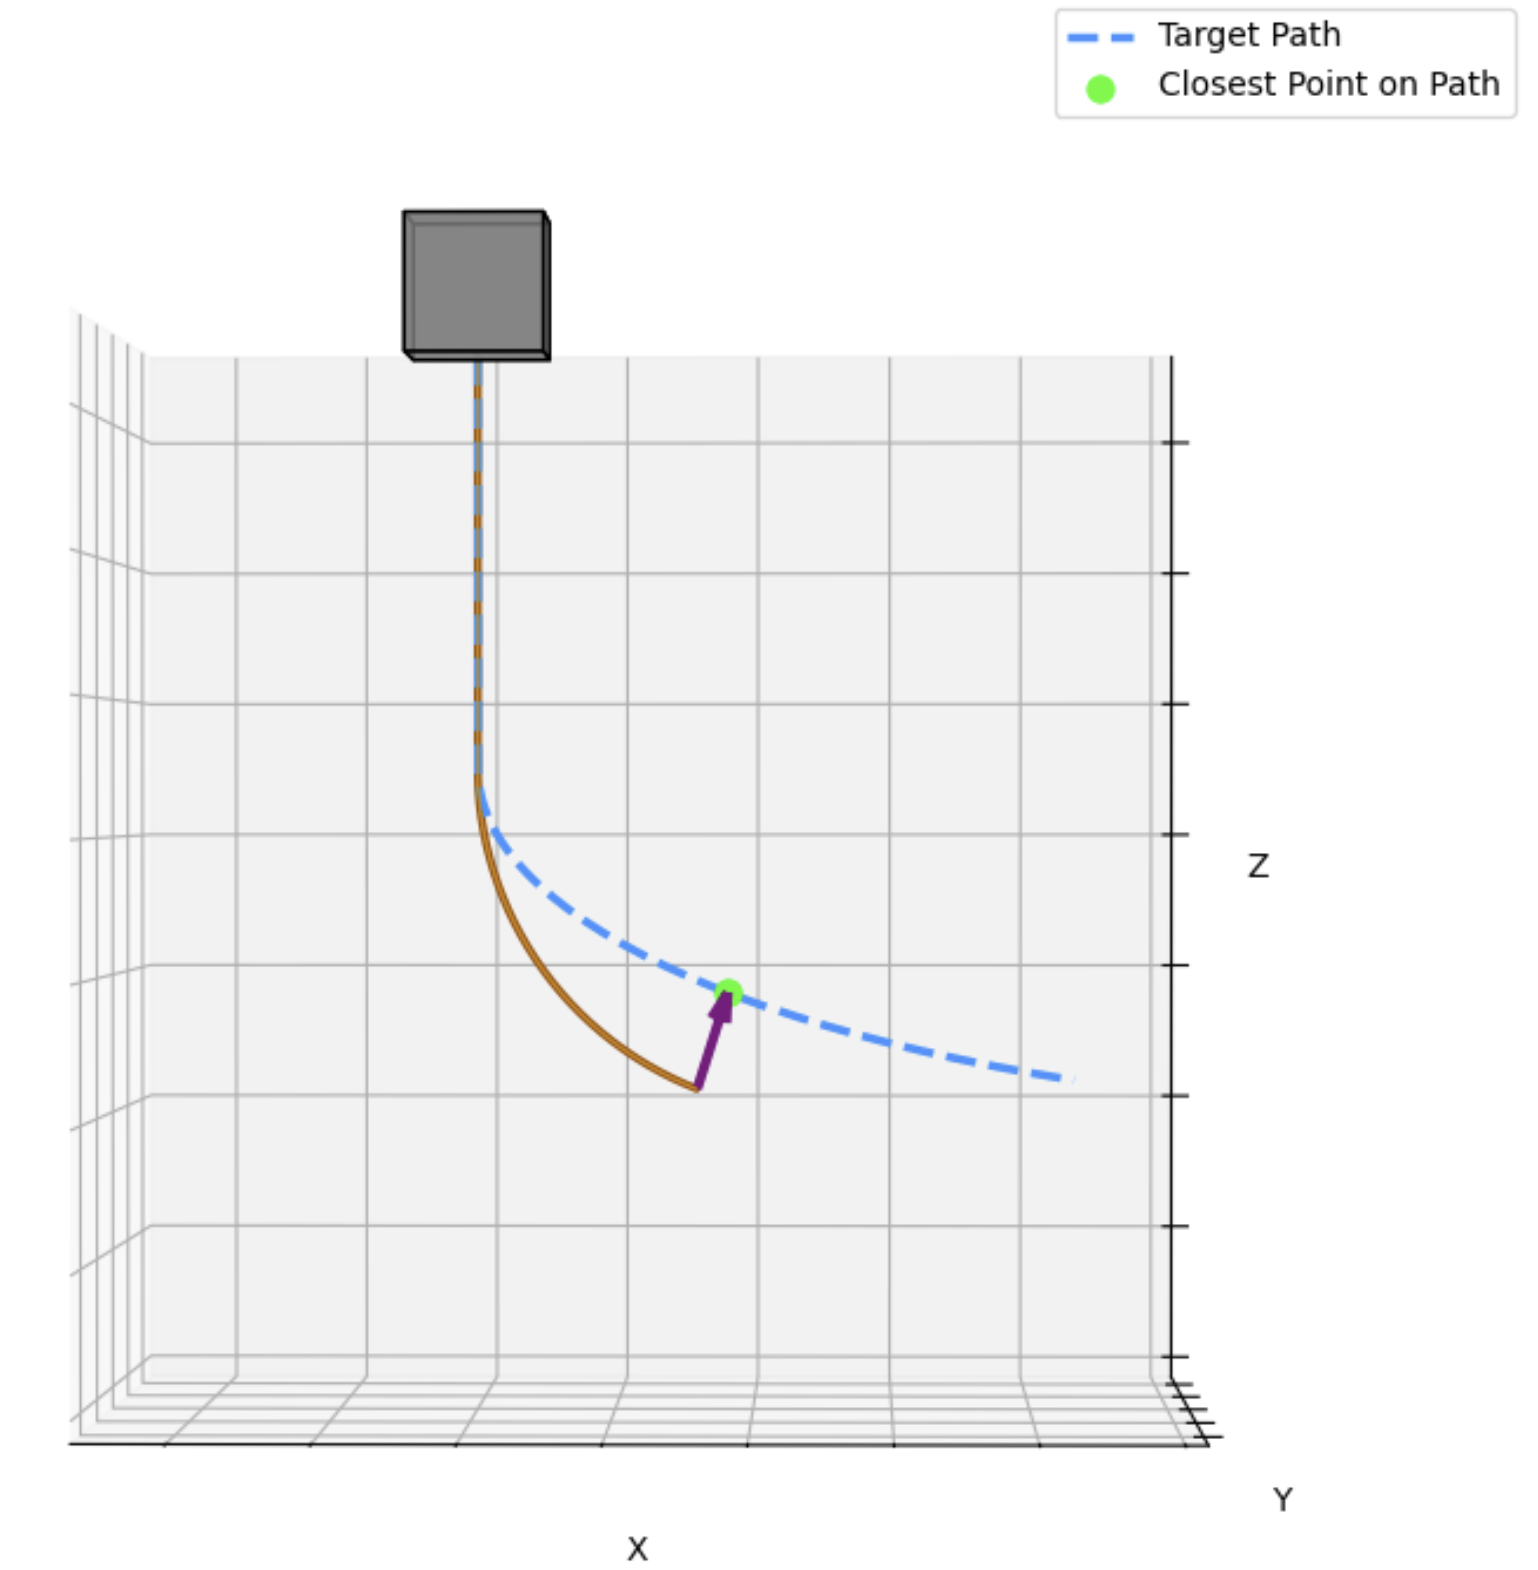
\includegraphics[width=0.7\linewidth]{images/pythonpictures/purepursuit.png}
    \caption{Visualization of orthogonal projection guidance (reference angle being the angle between z-axis and the purple arrow)}
    \label{fig:purepursuit}
\end{figure}
This approach is simple and intuitive. However, the convergence behavior may be problematic in practice. Since the controller always aims for the nearest point on the path it continues to generate turning commands even when the vehicle is nearly aligned. This causes overshooting and unnecessary steering corrections. Further, this method can encounter issues in certain geometric scenarios. Particularly on circular paths when the vehicle crosses the centerpoint of the curvature. In this case the projection onto the path is no longer well-defined and the method can break down \cite{fossen_handbook_2011}.

\paragraph*{Line of Sight}
The LOS guidance method is now widely used due to its small computational cost, easy implementation and intuitiveness \cite{qi_curve_2022} \cite{caharija_integral_2016}. Instead of using the closest point on the path, LOS guidance steers the vehicle toward a point located a fixed distance ahead on the path (known as the lookahead distance). In effect it imitates a helmsman steering the vessel toward a point lying at a constant distance ahead of the ship along the desired path \cite{caharija_integral_2016}. In the case of no enivronmental disturbances, simple LOS has good path convergence properties \cite{borhaug_integral_2008}. 
\begin{figure} [H]
    \centering
    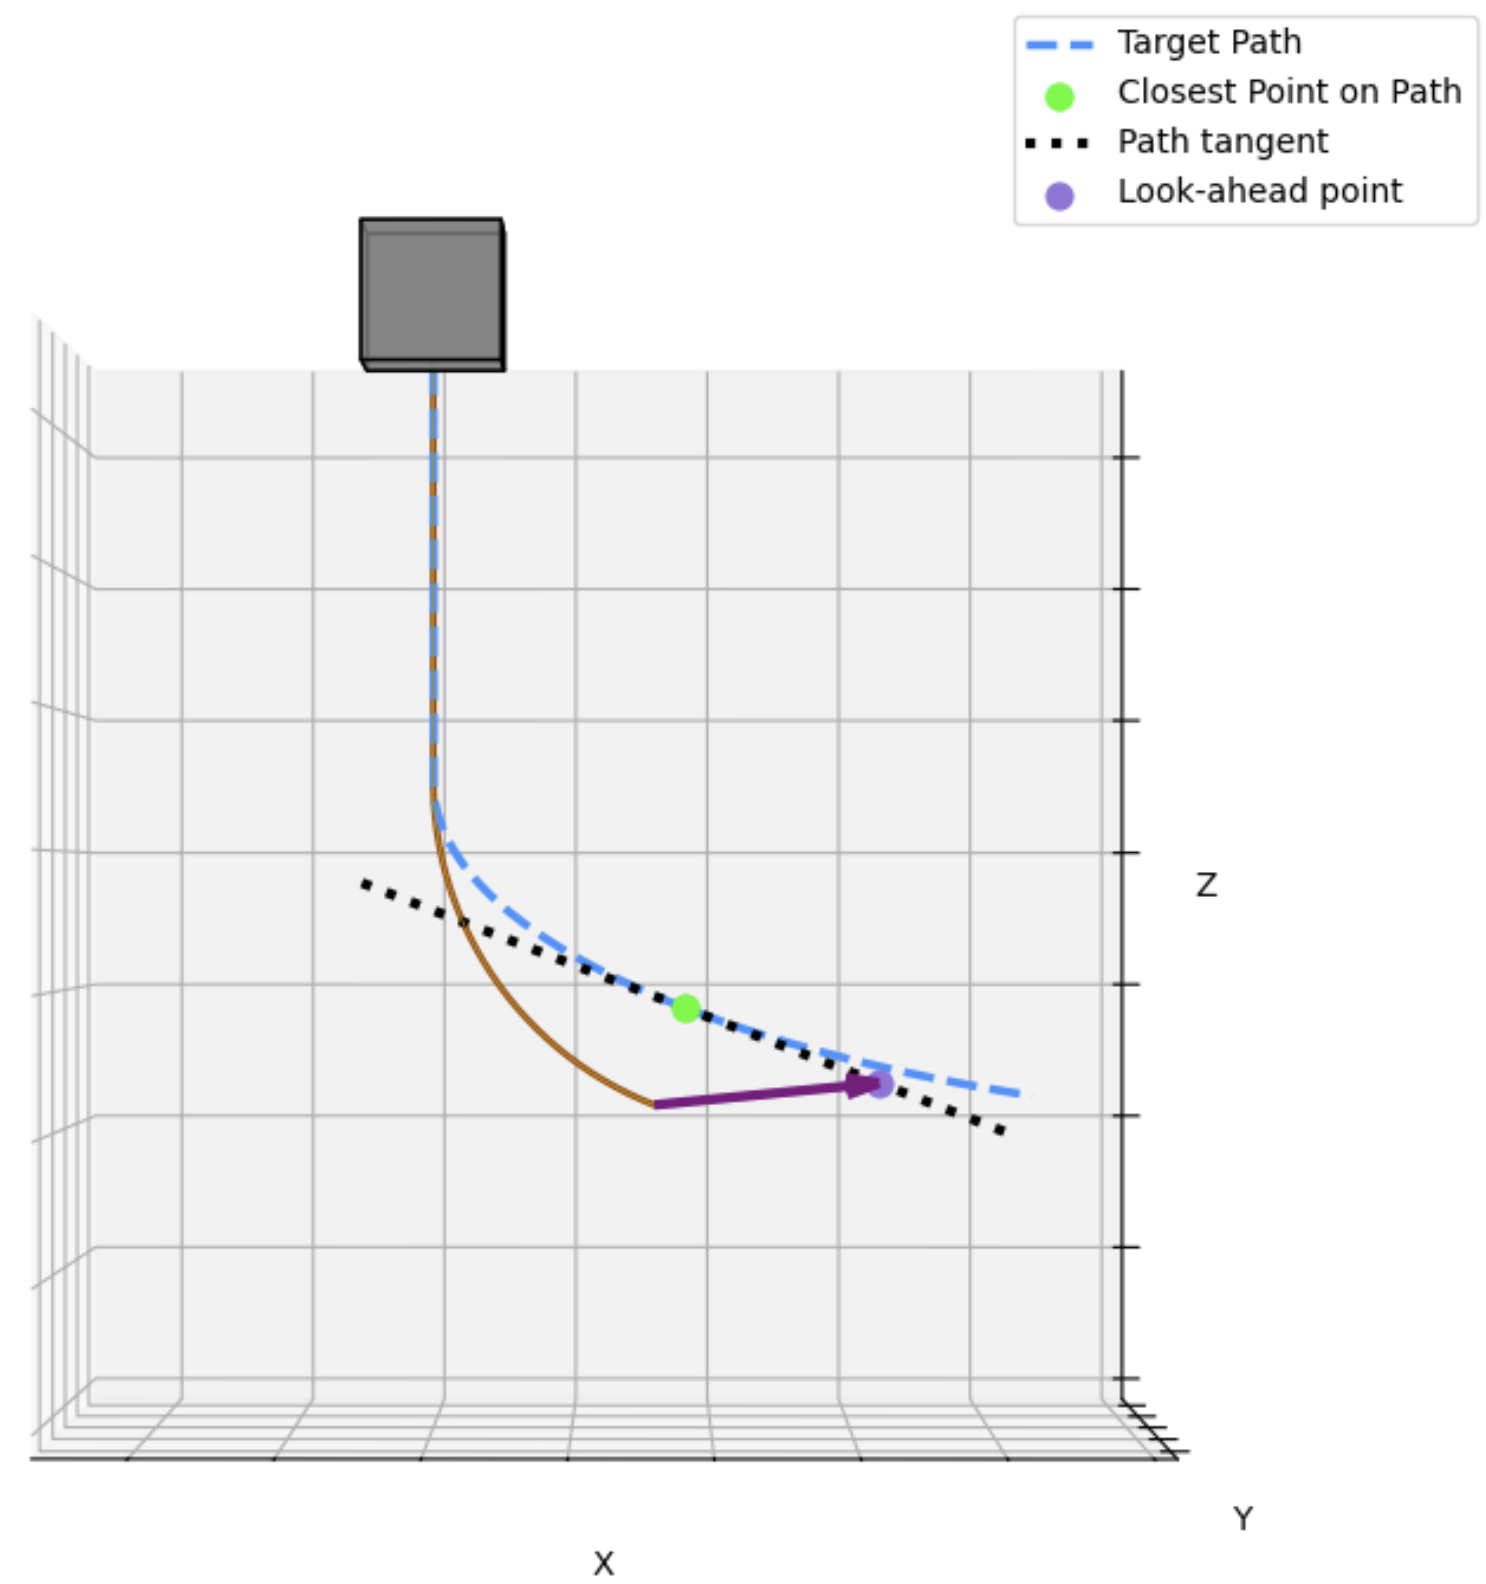
\includegraphics[width=0.7\linewidth]{images/pythonpictures/LOS.png}
    \caption{Visualization of LOS guidance (the angle between the z-axis and the purple arrow becomes the reference pitch angle)}
    \label{fig:LOS}
\end{figure}
However, path following control approaches based on traditional LOS guidance are susceptible to environmental disturbances \cite{borhaug_integral_2008} or more generally all errors that case the actual navigation direction to differ from the guidance direction. In particular this will lead to path deviation and convergence problems \cite{borhaug_integral_2008}. Moreover, this drawback cannot be fixed by simply adding integral action to the heading controller, the problem originates from the heading reference generator, that is, the LOS guidance law itself \cite{borhaug_integral_2008}.

\paragraph*{Integral Line of Sight (ILOS)}
To address the limitation of traditional LOS, Børghaug et al. \cite{borhaug_integral_2008} proposed a guidance law based on the LOS guidance principle but that includes integral action to overcome the drawbacks of environmental disturbance while preserving the intuition and the simplicity of traditional LOS guidance.
\begin{figure} [H]
    \centering
    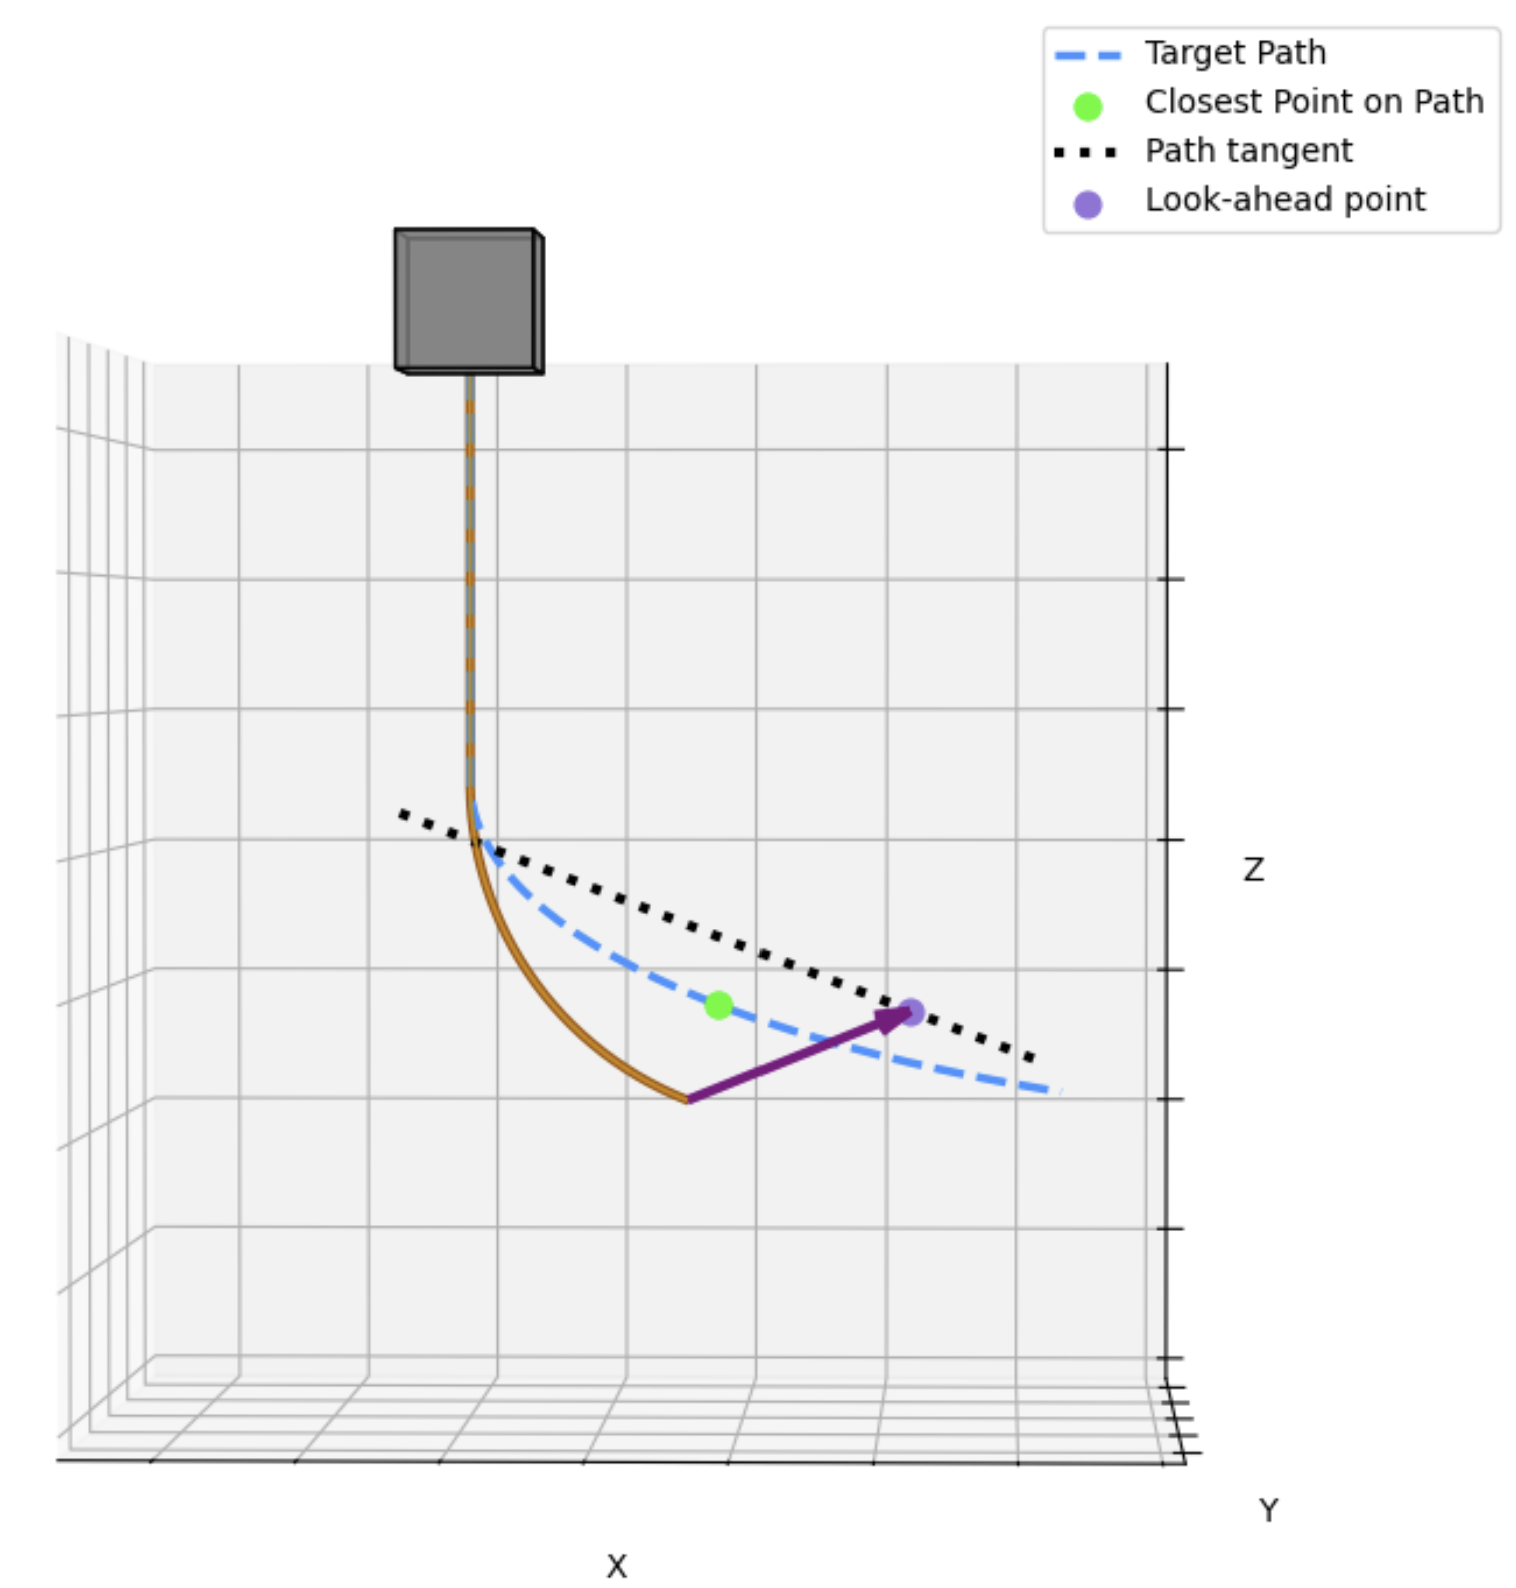
\includegraphics[width=0.7\linewidth]{images/pythonpictures/ILOS.png}
    \caption{Visualization of ILOS guidance (the angle between the z-axis and the purple arrow becomes the reference pitch angle)}
    \label{fig:ILOS}
\end{figure}
By integrating the cross-track error over time, ILOS effectively reduces steady-state error and restores path convergence even when the vessels actual movement direction deviates from its commanded heading.

\paragraph*{Adaptive Methods}
Adaptive guidance methods can improve path-following in uncertain or dynamic environments by adjusting parameters in real time. Several adaptive approaches have been adopted for path-following including adaptive LOS \cite{fossen_direct_2017}, where for example the look-ahead distance is varied based on cross-track error \cite{lekkas_integral_2014} or path curvature \cite{liu_path_2017}, \cite{hung_review_2023}. This allows the system to steer more smoothly when far from the path and more precisely when close, reducing overshooting and unnecessary correction.
\newline \newline 
Other methods include adaptive vector field guidance which modifies the synthetic vector field used to steer the vehicle toward the path \cite{wang_adaptive_2022} \cite{wang_adaptive_2022}. By adjusting the shape or strength of the filed based on real-time errors or estimated disturbances \cite{soetanto_adaptive_2003}. Or other techniques including sliding mode control \cite{soetanto_adaptive_2003} \cite{dagci_path_2003}, Learning-based MPC \cite{noauthor_learningbased_nodate}, \cite{rokonuzzaman_effective_2023} and reinforcement learning based control \cite{wang_path_2024}, \cite{martinsen_reinforcement_2020}, \cite{hung_review_2023}.

\paragraph*{Model Predicitve Control (MPC)}
Model Predictive Control (MPC) is an optimization-based approach that computes control actuation by predicting future system behavior over a finite time horizon. At each time step, it solves and optimal control problem that minimizes path-following error while satisfying system constraints such a speed, turnign limits, and actuator bounds \cite{hung_review_2023}. 
\newline \newline
Unlike geometric methods like LOS or pure pursuit, MPC can explicitly handle physical constraints and nonlinear dynamics. Linear model predictive control \cite{kanjanawanishkul_mpc-based_2015}, nonlinear MPC \cite{guo_model_2019} \cite{xu_model_2021} and learning-based MPC have all been used in path following research \cite{hung_review_2023}. However they are complicated in terms of design and implementation since they involve solving an optimization problem online. Yet since they deal with the vehicle's input constraints i.e. velocity and angular rate explicitly they are  expected to outperform other path following strategies in cases that require the vehicle to maneuver more aggressively. Another advantage is that they can incorporate more easily other tasks such as obstacle avoidance in the path following problem. Although using these methods is particularly challenging in environments and with devices that are not easily modeled.

\lhead{2D Path following - Design} % section header
\subsection{Design}

\subsubsection{Choice of Kinematic Modeling Approach}
In the background chapter, several approached previously applied to modeling steerable needles were presented including 2D \cite{ko_two-dimensional_2010} and 3D unicycle models \cite{secoli_closed-loop_2013} as well as bicycle models \cite{webster_nonholonomic_2006} \cite{fallahi_extended_2015}. Based on this review and the physical differences between the ribbon device and the steerable needles a choice was made to begin with a 2D model inspired by the programmable bevel-tip needle work of Ko et al. \cite{ko_two-dimensional_2010}.This model has shown to be effective for steerable needles in soft tissue and its simplicity makes it a good starting off point. If the performance of this method proves insufficient another, more complex model may be adopted later.

\subsubsection{Final 2D Kinematic model}
As mentioned in the hardware section the ribbon device is moved up and down i.e. in the z-plane via control of the linear stage which is attatched at the proximal tip of the device. However movement in the x and y plane is controlled via controlling the tensions at the tendons which are attached to motors at the top and the tip of the ribbon at the bottom. When the ribbon is inserted in a brain phantom via the movement of the linear stage its trajectory will depend on the deflection of the tip. Which is in turn dependent on the tendon activation pattern which results in the bending or twisting of the tip. 
\newline \newline
To capture this behavior a unicycle type model inspired by \cite{ko_two-dimensional_2010} is used where the tip orientation is described using an Euler angle representation, which describes the orientation between the global frame and the local body coordinate frame as three rotations: roll \(\phi\), pitch \(\theta\) and yaw \(\psi\) which represent rotations about the local body cartesian axes \(x\), \(y\) and \(z\) respectively.

\begin{figure} [H]
    \centering
    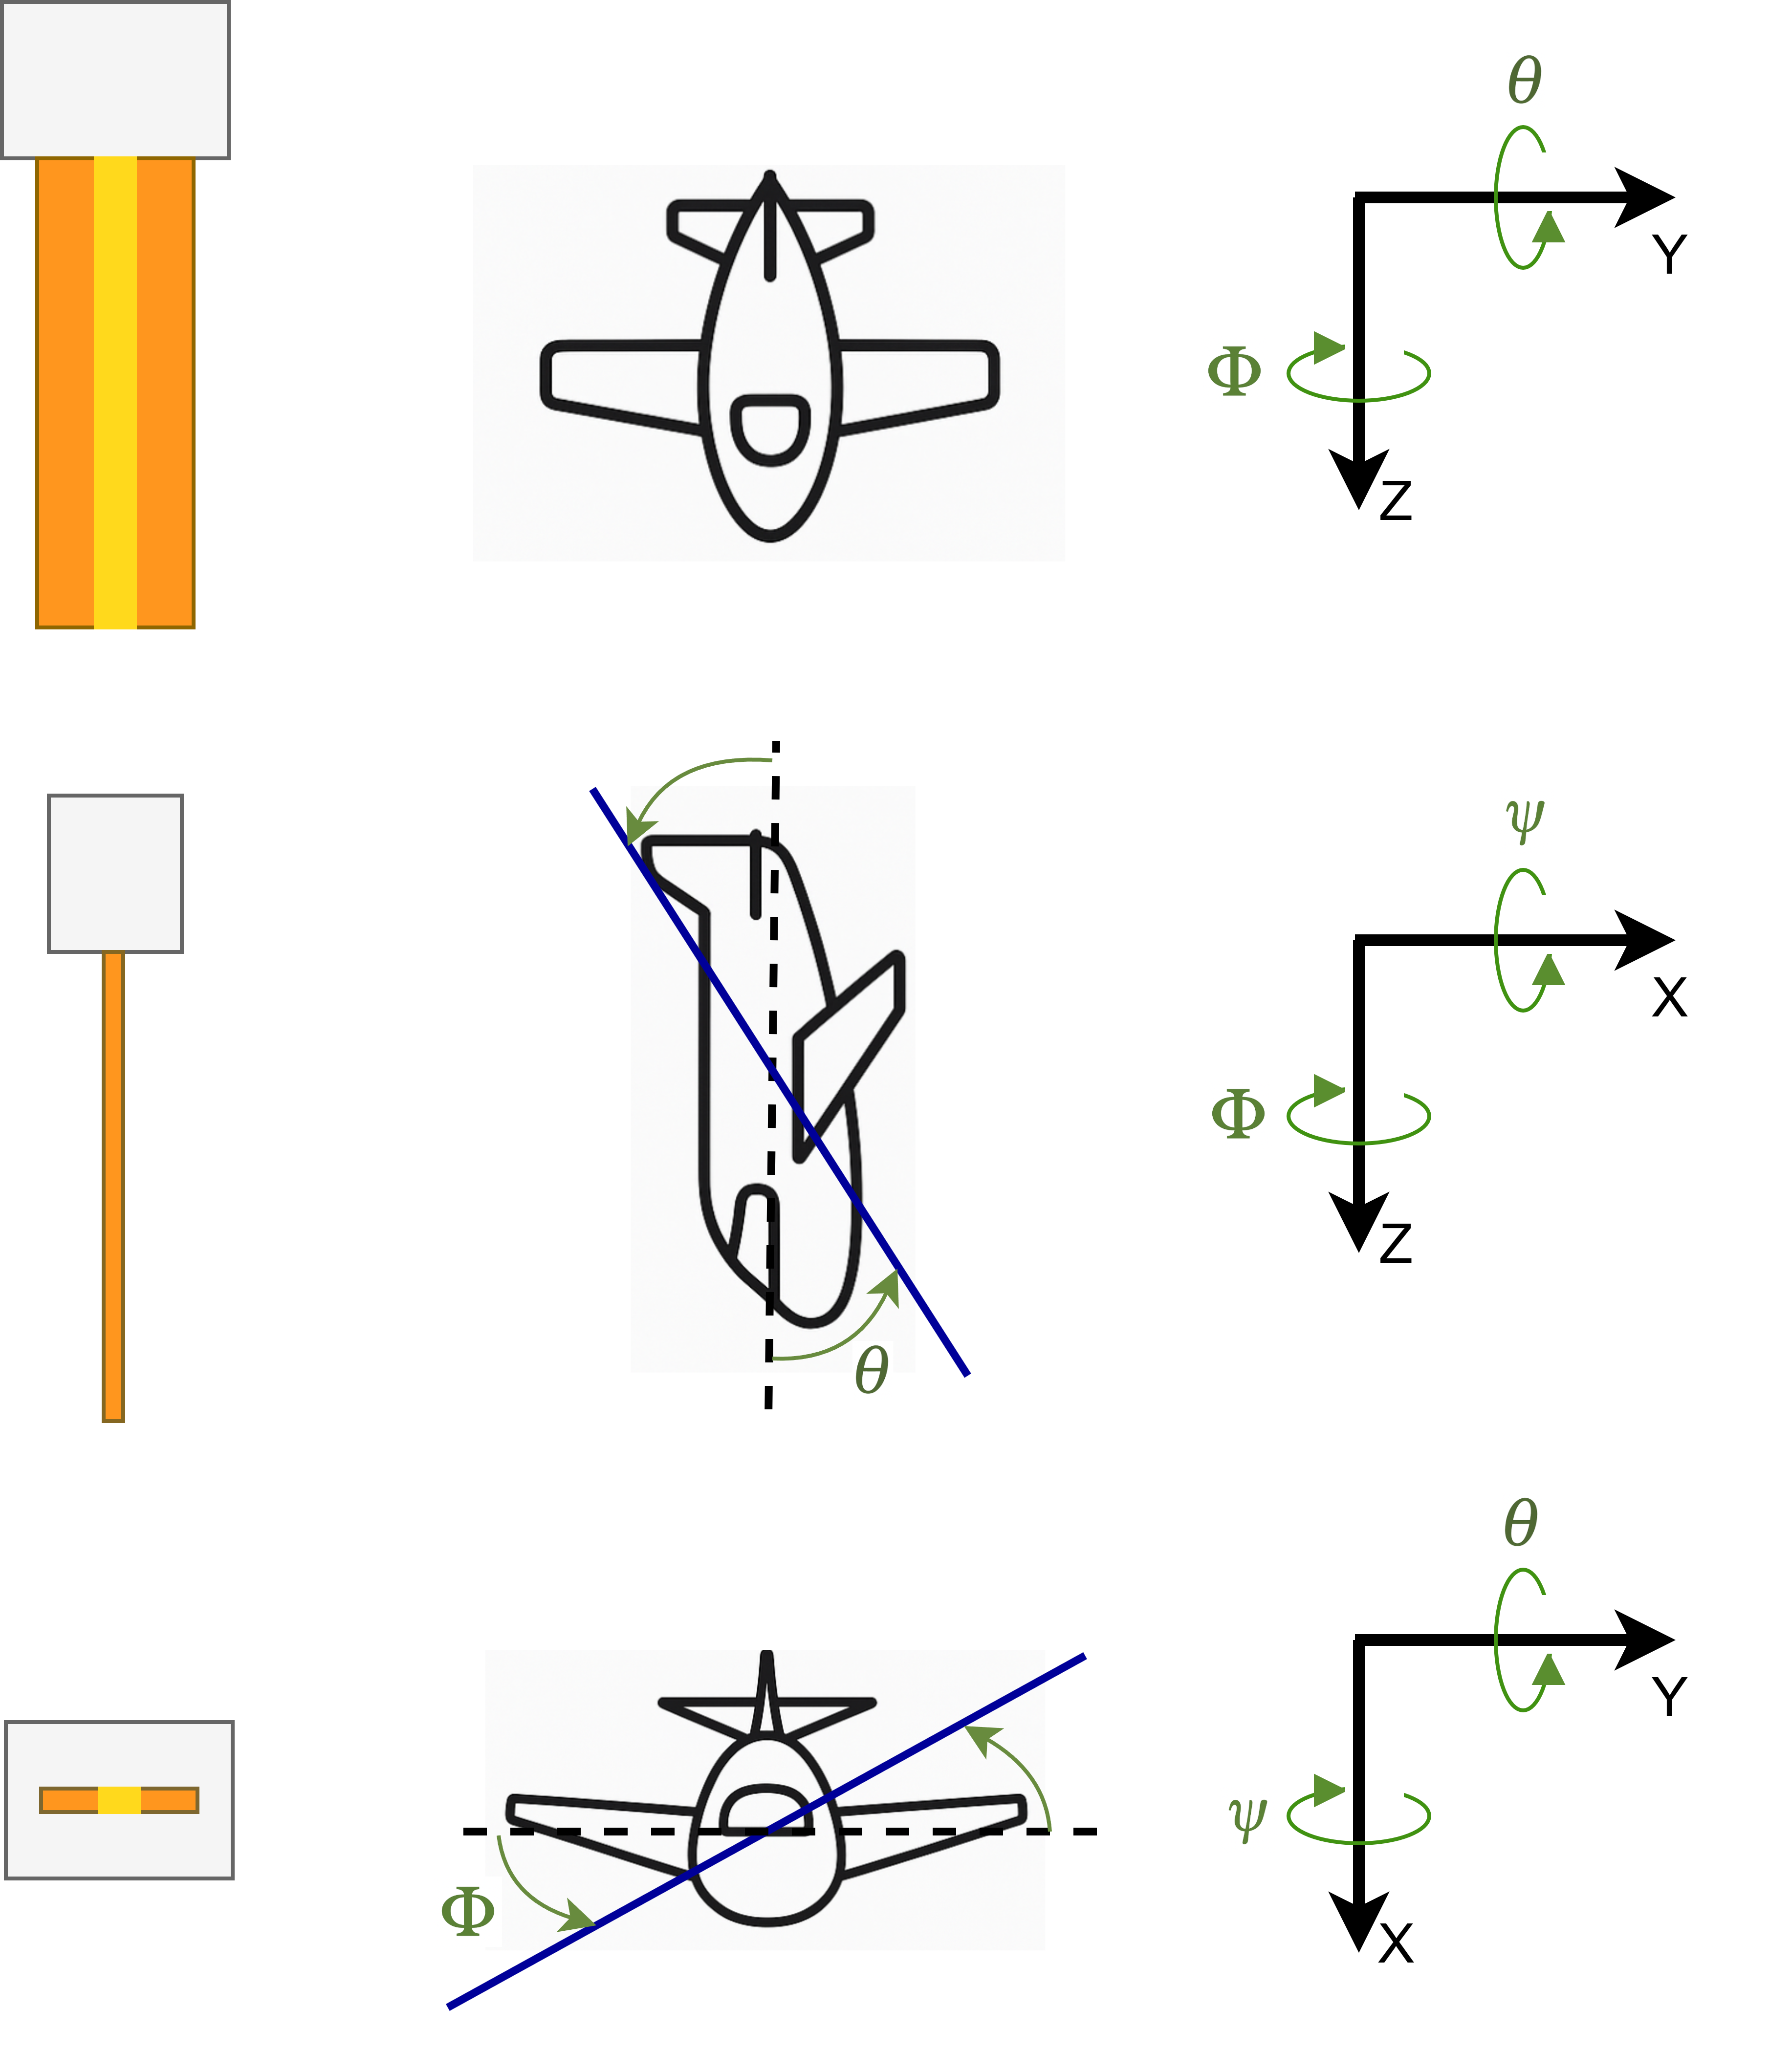
\includegraphics[width=0.7\linewidth]{images/planes.png}
    \caption{Visualization of the definition of Euler angles for the ribbon system and its analogy to vehicle models}
    \label{fig:planes}
\end{figure}



In the 2D kinematic model we assume the global y-position to be constant and thus there is no velocity component along that axis. When the tip bends in order to follow a trajectory it is performing a rotation around the local y-axis in the x-z-plane as is visualized in figure \ref{fig:theta} and \ref{fig:planes}. The rotational matrix thereby becomes

\begin{equation}
    \textbf{R} = \textbf{R}(\theta) = \begin{bmatrix}
        cos \theta   &   0   &   -sin \theta \\
        0            &   1   &   0\\
        sin \theta   &   0   &   cos \theta
    \end{bmatrix}
\end{equation}

\begin{figure} [H]
    \centering
    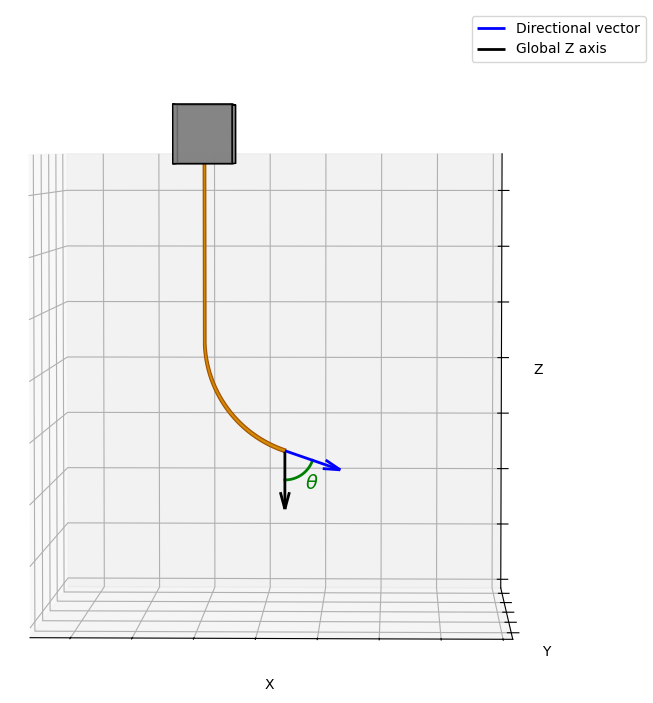
\includegraphics[width=0.55\linewidth]{images/pythonpictures/Capture.PNG}
    \caption{Visualization of the $\theta$ angle the determines the rotation around the local y-axis}
    \label{fig:theta}
\end{figure}
and the kinematic model becomes
\begin{equation}
    \vec{v_g} = \textbf{R}(\theta) \vec{v_b}
\end{equation}
Where $\vec{v_g}$ signifies the velocity of the tip in the global frame, \textbf{R}$\theta$ is the rotational matrix around the y-axis that transforms the body velocity of the tip of the ribbon given in the body frame $\vec{v_b}$ to the global frame. Inserting the previously defined rotational matrix we have:
\begin{equation}
    \begin{bmatrix}
        \dot{x}\\ \dot{y}\\ \dot{z}
    \end{bmatrix} = 
    \begin{bmatrix}
        cos \theta   &   0   &   -sin \theta \\
        0            &   1   &   0\\
       -sin \theta   &   0   &   cos \theta
    \end{bmatrix}
    \begin{bmatrix}
        v_x^b \\ v_y^b \\ v_z^b
    \end{bmatrix}
\end{equation}

\begin{equation}
    \begin{bmatrix}
        \dot{x}\\ \dot{y}\\ \dot{z}
    \end{bmatrix} = \begin{bmatrix}
        v_x^bcos \theta - v_z^b sin \theta\\
        v_y^b\\
        v_x^b sin \theta  v_z^b cos \theta
    \end{bmatrix}
\end{equation}
However since we are in the 2D case where \(v_y^b = 0\) we can simplify this to:
\begin{equation}
        \begin{bmatrix}
        \dot{x}\\ \dot{z}
    \end{bmatrix} = \begin{bmatrix}
        v_x^bcos \theta - v_z^b sin \theta\\
        v_x^b sin \theta + v_z^b cos \theta
    \end{bmatrix}
\end{equation}
Further since the ribbon is inserted via the linear stage moving the backbone down the velocity along the ribbons z-axis will be the only significant velocity component in a stiff medium, therefore we can further simplify the model to.
\begin{equation}
	\begin{bmatrix}
	\dot{x} \\ \dot{z}
	\end{bmatrix} = \begin{bmatrix}
	-sin\theta \\ cos\theta
	\end{bmatrix} v_z^b
\end{equation}

\begin{figure} [H]
    \centering
    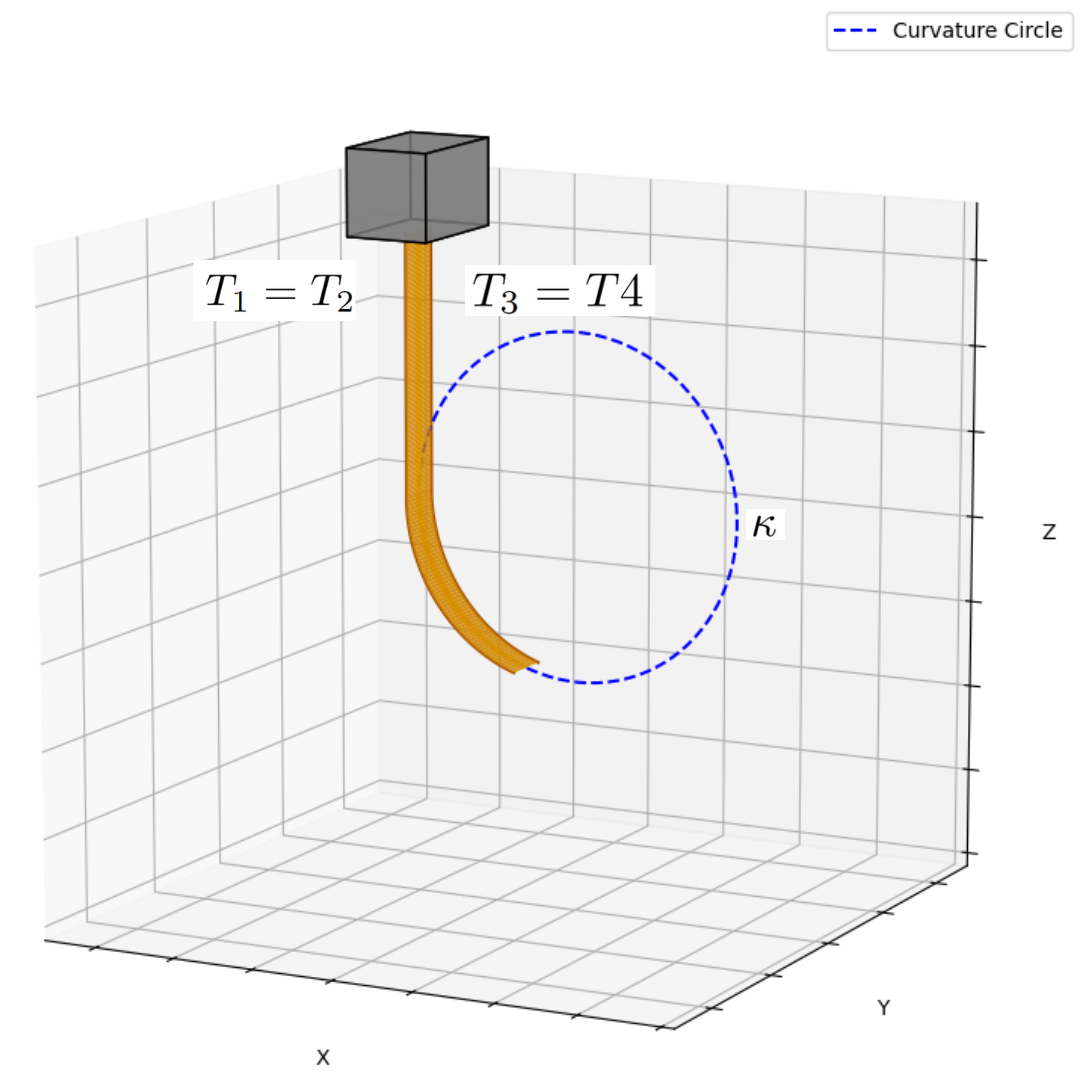
\includegraphics[width=0.6\linewidth]{images/pythonpictures/curvature.PNG}
    \caption{Visualization of how the curvature of the tip $\kappa$ controlled by the difference in tension on the left side \(T_1, T_2\) and right \(T_3, T_4\) influences the trajectory of the ribbon}
    \label{fig:curvature}
\end{figure}

In terms of the rotational velocity, it is defined by the relationship between the instantaneous curvature $\kappa$ at the tip and the insertion velocity $v_z^b$. Since 
\begin{equation}
    \frac{d}{dt}\theta  = \frac{d\theta}{ds}\frac{ds}{dt}=\kappa v_z^b
\end{equation}

The instantaneous curvature $\kappa_{tip}$, visualized in figure \ref{fig:curvature} is further assumed to be a function of the difference in tension between the tendons on the right and left side $f(u)$, which is given by the actuation variable defined as $u$. Where $f(u)$ is a monotonically increasing function of the actuation variable. In this project this is simplified to be a linear function, independent of previous states and defined by only the offset $b$ and the slope $a$. 
\begin{equation}
	\kappa_{tip} = f(u) = a\cdot u + b
\end{equation}

Including the angular velocity in the system model we arrive at the final 2D model:
\begin{equation}
	\begin{bmatrix}
		\dot{x} \\ \dot{z} \\ \dot{\theta}
	\end{bmatrix} = \begin{bmatrix}
	-sin\theta \\ cos\theta \\ f(u)
	\end{bmatrix}v_z^b
\end{equation}



\subsubsection{Final 2D Control System Design}

\begin{figure} [H]
    \centering
    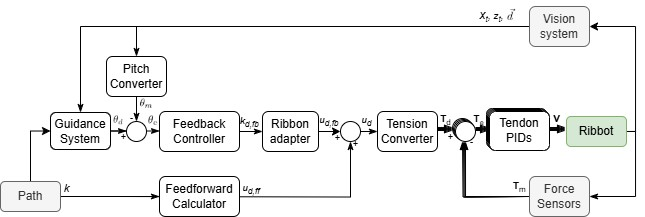
\includegraphics[width=\linewidth]{images/RibbotControl_V2.png}
    \caption{Full control system diagram for 2D path following}
    \label{fig:2Dcontrol}
\end{figure}
A visualization of the full control system architecture for 2D path following is shown in figure \ref{fig:2Dcontrol}. The system uses a predefined spatial path as reference (see Path Planning Integration chapter) and continuously adjusts the tendon tensions to steer the ribbon tip along this path. The current position \((x_t, z_t)\) is extracted from vision data (see Tip Tracking Integration chapter) and passed to the \texttt{GuidanceSystem}, which computes the desired pitch angle \(\theta_d\). The orientation of the tip \(\vec{d}\) is also extracted from the vision data and passed to the \texttt{PitchConverter} which calculates the measure pitch angle \(\theta_m\). The desired pitch angle \(\theta_d\) is then compared to the measured pitch angle \(\theta_m\), and the resulting error \(\theta_e\) is used by the feedback controller, here a PI controller to compute a corrective curvature command \(\kappa_{d,fb}\) which in this system corresponds to how fast the pitch changes as the ribbon advances in space since 
\begin{equation}
    \kappa = \frac{d\theta}{ds}
\end{equation}
Before any path following is done the ribbon is run through a calibration protocol where its bending dynamics based on tendon tension are mapped, after this has been mapped the user inputs this into the gui and the \texttt{RibbonAdapter} module that receives the desired corrective \(\kappa_{d, fb}\) uses this in order to calculate the appropriate actuation value \(u_{d, fb}\) in order to achieve the desired curvature for this particular ribbon. The actuation value \(u\) is defined as 
\begin{equation}
    u = T_{3,4} - T_ {1,2}
\end{equation}
Where \(T_{3,4}\) corresponds to the tension on tendon 3 and 4 which are placed on the right side, and \(T_{1,2}\) corresponds to the tension on tendon 1 and 2 which are on the left side. 
\newline \newline
To assist the controller and improve responsiveness, a feedforward signal based on the local path curvature at the closest point is calculated by the \texttt{FeedbackCalculator} modulate. This feedbackterm \(u_{d, ff}\) is then combined with the feedback term and sent to the \texttt{TensionConverter} module. This module converts that actuation value into individual tendon tension targets \(\textbf{T}_d\) based on a set of rules which ensure a baseline tension is maintained and tension limits aren't exceeded. These targets are then sent to the low-level tension controllers (see closed-loop tension control chapter) which ensure that the tendons track their tension targets using feedback from force sensors.



\subsubsection{Choice of Guidance system}
The chosen path-following strategy must above all be reliable, modular and suit the constraints of the ribbon-based system. Among the available options, pure pursuit, LOS, ILOS, adaptive and MPC, the initial chosen strategy is LOS guidance is it is a simple yet very effective solution to path following.
\newline \newline 
Although more advanced techniques such as MPC or adaptive control could provide better performance in theory, they are currently impractical for this system. In particular, implementing MPC poses significant challenges because of the highly nonlinear and complex dynamics of the ribbon. The tendon actuation results in strong coupling between degrees of freedom and the deformation fo the ribbon is influenced by wear, material hysteresis, buckling and loading history. The future surgical environment adds another layer of complexity through contact forces with tissue that are difficult to predict and incorporate into the optimization framework. All of which make it extremely difficult to develop an accurate predictive model required for MPC.
\newline \newline
For these reasons, LOS offers a better, more practical solution. LOS is relatively straightforward to implement and has good convergence properties in undisturbed environments. It is also very easy to expand upon by adding a integral term, creating a ILOS guidance system that would better handle disturbances. It can even be made adaptive by making the look-ahead distance change based on chosen factors such as curvature or cross-track error. It is therefore a good starting off point for the system.

\subsubsection{Final LOS Guidance System Design}
As discussed in the chapter on the final 2D kinematic model of the ribbon the spatial position of the tip of the ribbon is represented by \(P(t) \triangleq [x(t), z(t)]^T\) and its velocity is \(v(t) \triangleq \dot{P}(t)\), stated relative to the stationary global frame. The speed is represented by \(U(t) \triangleq |v(t)| = \sqrt{\dot{x}(t)^2 + \dot{z}(t)^2}\). The steering is characterized the angular variable \(\theta(t) \triangleq atan2(\dot{x}(t), \dot{z}(t))\) (visualized in figure \ref{fig:theta}). Path following is then ensured by proper assignments to \(\theta(t)\).
\newline \newline
In the final LOS guidance system design we consider a planar path continuously parameterized by a scalar variable, \(\epsilon\), such that the position of a point belonging to the path is represented by \(P_p(\epsilon) \triangleq [x_p(\epsilon), z_p(\epsilon)]^T\). Subsequently we consider an arbitrary path point \(P_p(\epsilon)\) and define a path-fixed reference frame with origin at this point. Then starting with the same orientation as the global stationary frame, a simple elementary rotation can be performed to arrive at this path-fixed frame. This is done by rotating the stationary frame by the path-tangential angle
\begin{equation}
    \zeta_p(\epsilon) = atan2(x_p'(\epsilon), z_p'(\epsilon))
\end{equation}
about its y-axis, as is visualized in figure \ref{fig:pathframerotation}.

\begin{figure} [H]
    \centering
    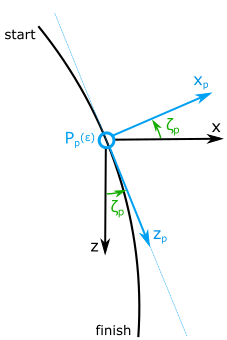
\includegraphics[width=0.4\linewidth]{images/inkscape/pathframeRotatione.png}
    \caption{Visualization of the rotation from the global stationary frame to the pathframe, characterized by the angle \(\zeta_p\)}
    \label{fig:pathframerotation}
\end{figure}

The rotation can also be represented by the rotation matrix
\begin{equation}
    R(\zeta_p) = \begin{bmatrix}
        cos\zeta_p & -sin\zeta_p \\
        sin \zeta_p & cos\zeta_p 
    \end{bmatrix}
\end{equation}
Such that the error decomposed in the path-fixed reference frame is given by
\begin{equation}
    e(t) = R(\zeta_p)^T(P(t) - P_p(\epsilon)) = [x_e(t), z_e(t)]^T
\end{equation}
where \(e(t) = [x_e(t), z_e(t)]^T\) represent the \textit{cross-track} and \textit{along-track} errors relative to \(P_p(\epsilon)\). The path following control objective thus becomes
\begin{equation}
    \lim_{t\to\infty} e(t) = 0
\end{equation}

However since \(P_p(\epsilon)\) is chosen by choosing \(\epsilon\) such that the Euclidean distance \(|P(t) - P_p(\epsilon)|\) is minimized, and the path is assumed to continuous, and smooth this corresponds to an orthogonal projection onto the path. Therefore the along-track error \(z_e(t)\) becomes negligible, i.e. \(z_e(t) \approx 0\), and only the cross-track error \(x_e(t)\) is used for guidance. and the control objective can be simplified to 
\begin{equation}
    \lim_{t \to \infty} x_e(t) = 0
\end{equation}
and this can be achieved by assigning appropriate steering law to \(P(t)\). 
\begin{figure} [H]
    \centering
    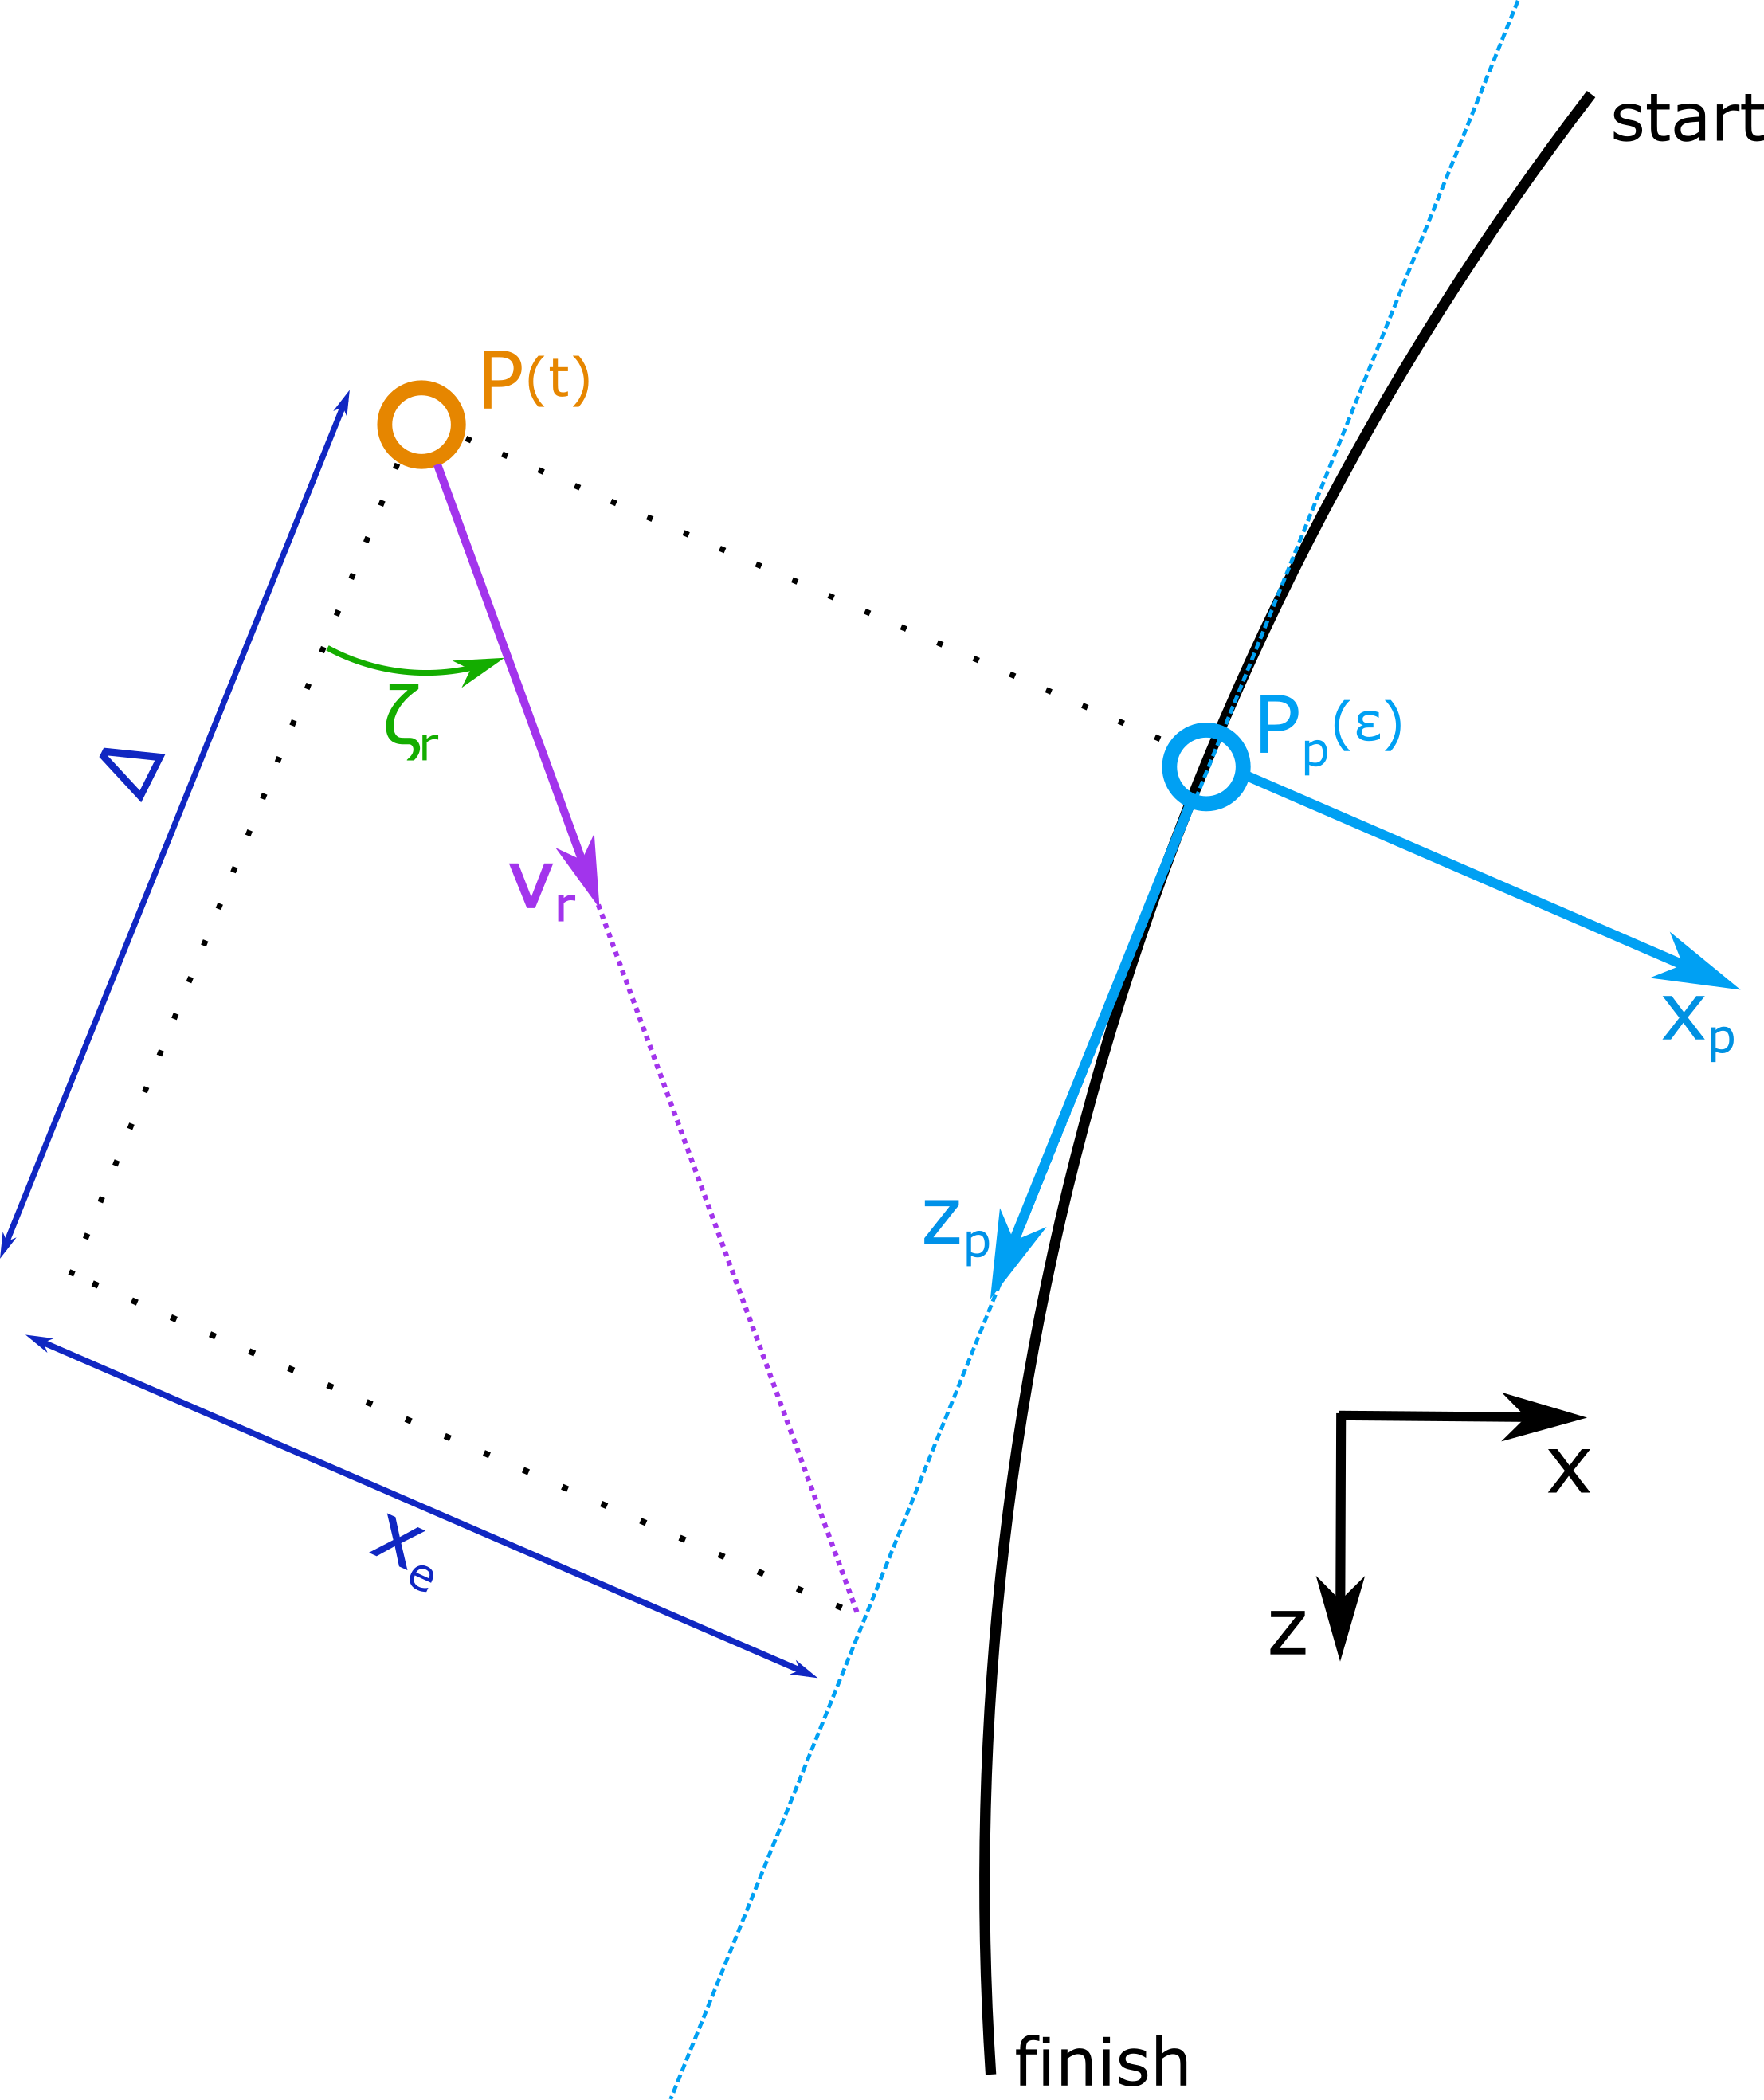
\includegraphics[width=0.65\linewidth]{images/inkscape/pathframee.png}
    \caption{Visualization of the variables associated with LOS steering for curved paths}
    \label{fig:pathframe}
\end{figure}
For the LOS case the LOS steering angle thus becomes
\begin{equation}
    \zeta_r(x_e) \triangleq arctan(-\frac{x_e(t)}{\Delta})
\end{equation}
where \(\zeta_r(x_e)\) is a velocity-path relative angle which ensures that the velocity is directed toward a point on the path that is located a \textit{lookahead distance} \(\Delta>0\) ahead of the direct projection of \(P(t)\) onto the path. See figure \ref{fig:pathframe}.


The rotation caused by \(\zeta_r(x_e)\) can also be represented by the rotation matrix 
\begin{equation}
    R(\zeta_r) = \begin{bmatrix}
        cos\zeta_r & -sin\zeta_r \\
        sin \zeta_r & cos\zeta_r
    \end{bmatrix}
\end{equation}

Another equally valid representation of the 2D kinematics written out in the section of the final 2D kinematic model thus becomes
\begin{equation}
    \begin{bmatrix}
        \dot{x} \\\dot{z}
    \end{bmatrix} = R(\zeta_p, \zeta_r)v_z^b = R(\zeta_p)R(\zeta_r)v_z^b
\end{equation}
\begin{equation}
    \begin{bmatrix}
        \dot{x} \\ \dot{z} 
    \end{bmatrix} = \begin{bmatrix}
        -cos\zeta_p sin\zeta_r + sin\zeta_p cos \zeta_r \\
        -sin\zeta_p sin \zeta_r + cos \zeta_p cos \zeta_r
    \end{bmatrix} v_z^b
\end{equation}
The final 2D steering angle is given by \(\theta_r(x_e)\), for a visualization of this angle see \ref{fig:theta}. Combining this steering angle with the previous equations we get that  \(\theta_r(t) = atan2(\dot{x}_r(t), \dot{z}_r(t)\)  becomes
\begin{equation}
    \theta_r(\zeta_p, \zeta_r) = atan2(-cos\zeta_p sin\zeta_r - sin\zeta_p cos \zeta_r, -sin\zeta_p sin \zeta_r + cos\zeta_pcos \zeta_r)
\end{equation}
which by geometrical simplification can be transformed to the more traditional formulation of LOS guidance
\begin{equation}
    \theta_r(\zeta_p, \zeta_r) = \zeta_p + \zeta_r
\end{equation}

\subsubsection{Final ILOS Guidance System Design}
The final design of the Integral-Line-Of-Sight (ILOS) guidance system builds heavily on the previously described LOS system, with the addition of an integral term when calculating the steering angle \(\zeta_r(x_e)\) (see figure \ref{fig:ilos}. Thus the new ILOS steering angle becomes:
\begin{equation}
    \zeta_{r}(x_e) \triangleq arctan(-\frac{x_e(t) +K_i\int x_e}{\Delta})
\end{equation}
Where \(K_i\) is a tunable design parameter, and integral gain and \(\Delta\) has the same interpretation as in the case of traditional LOS

\begin{figure} [H]
    \centering
    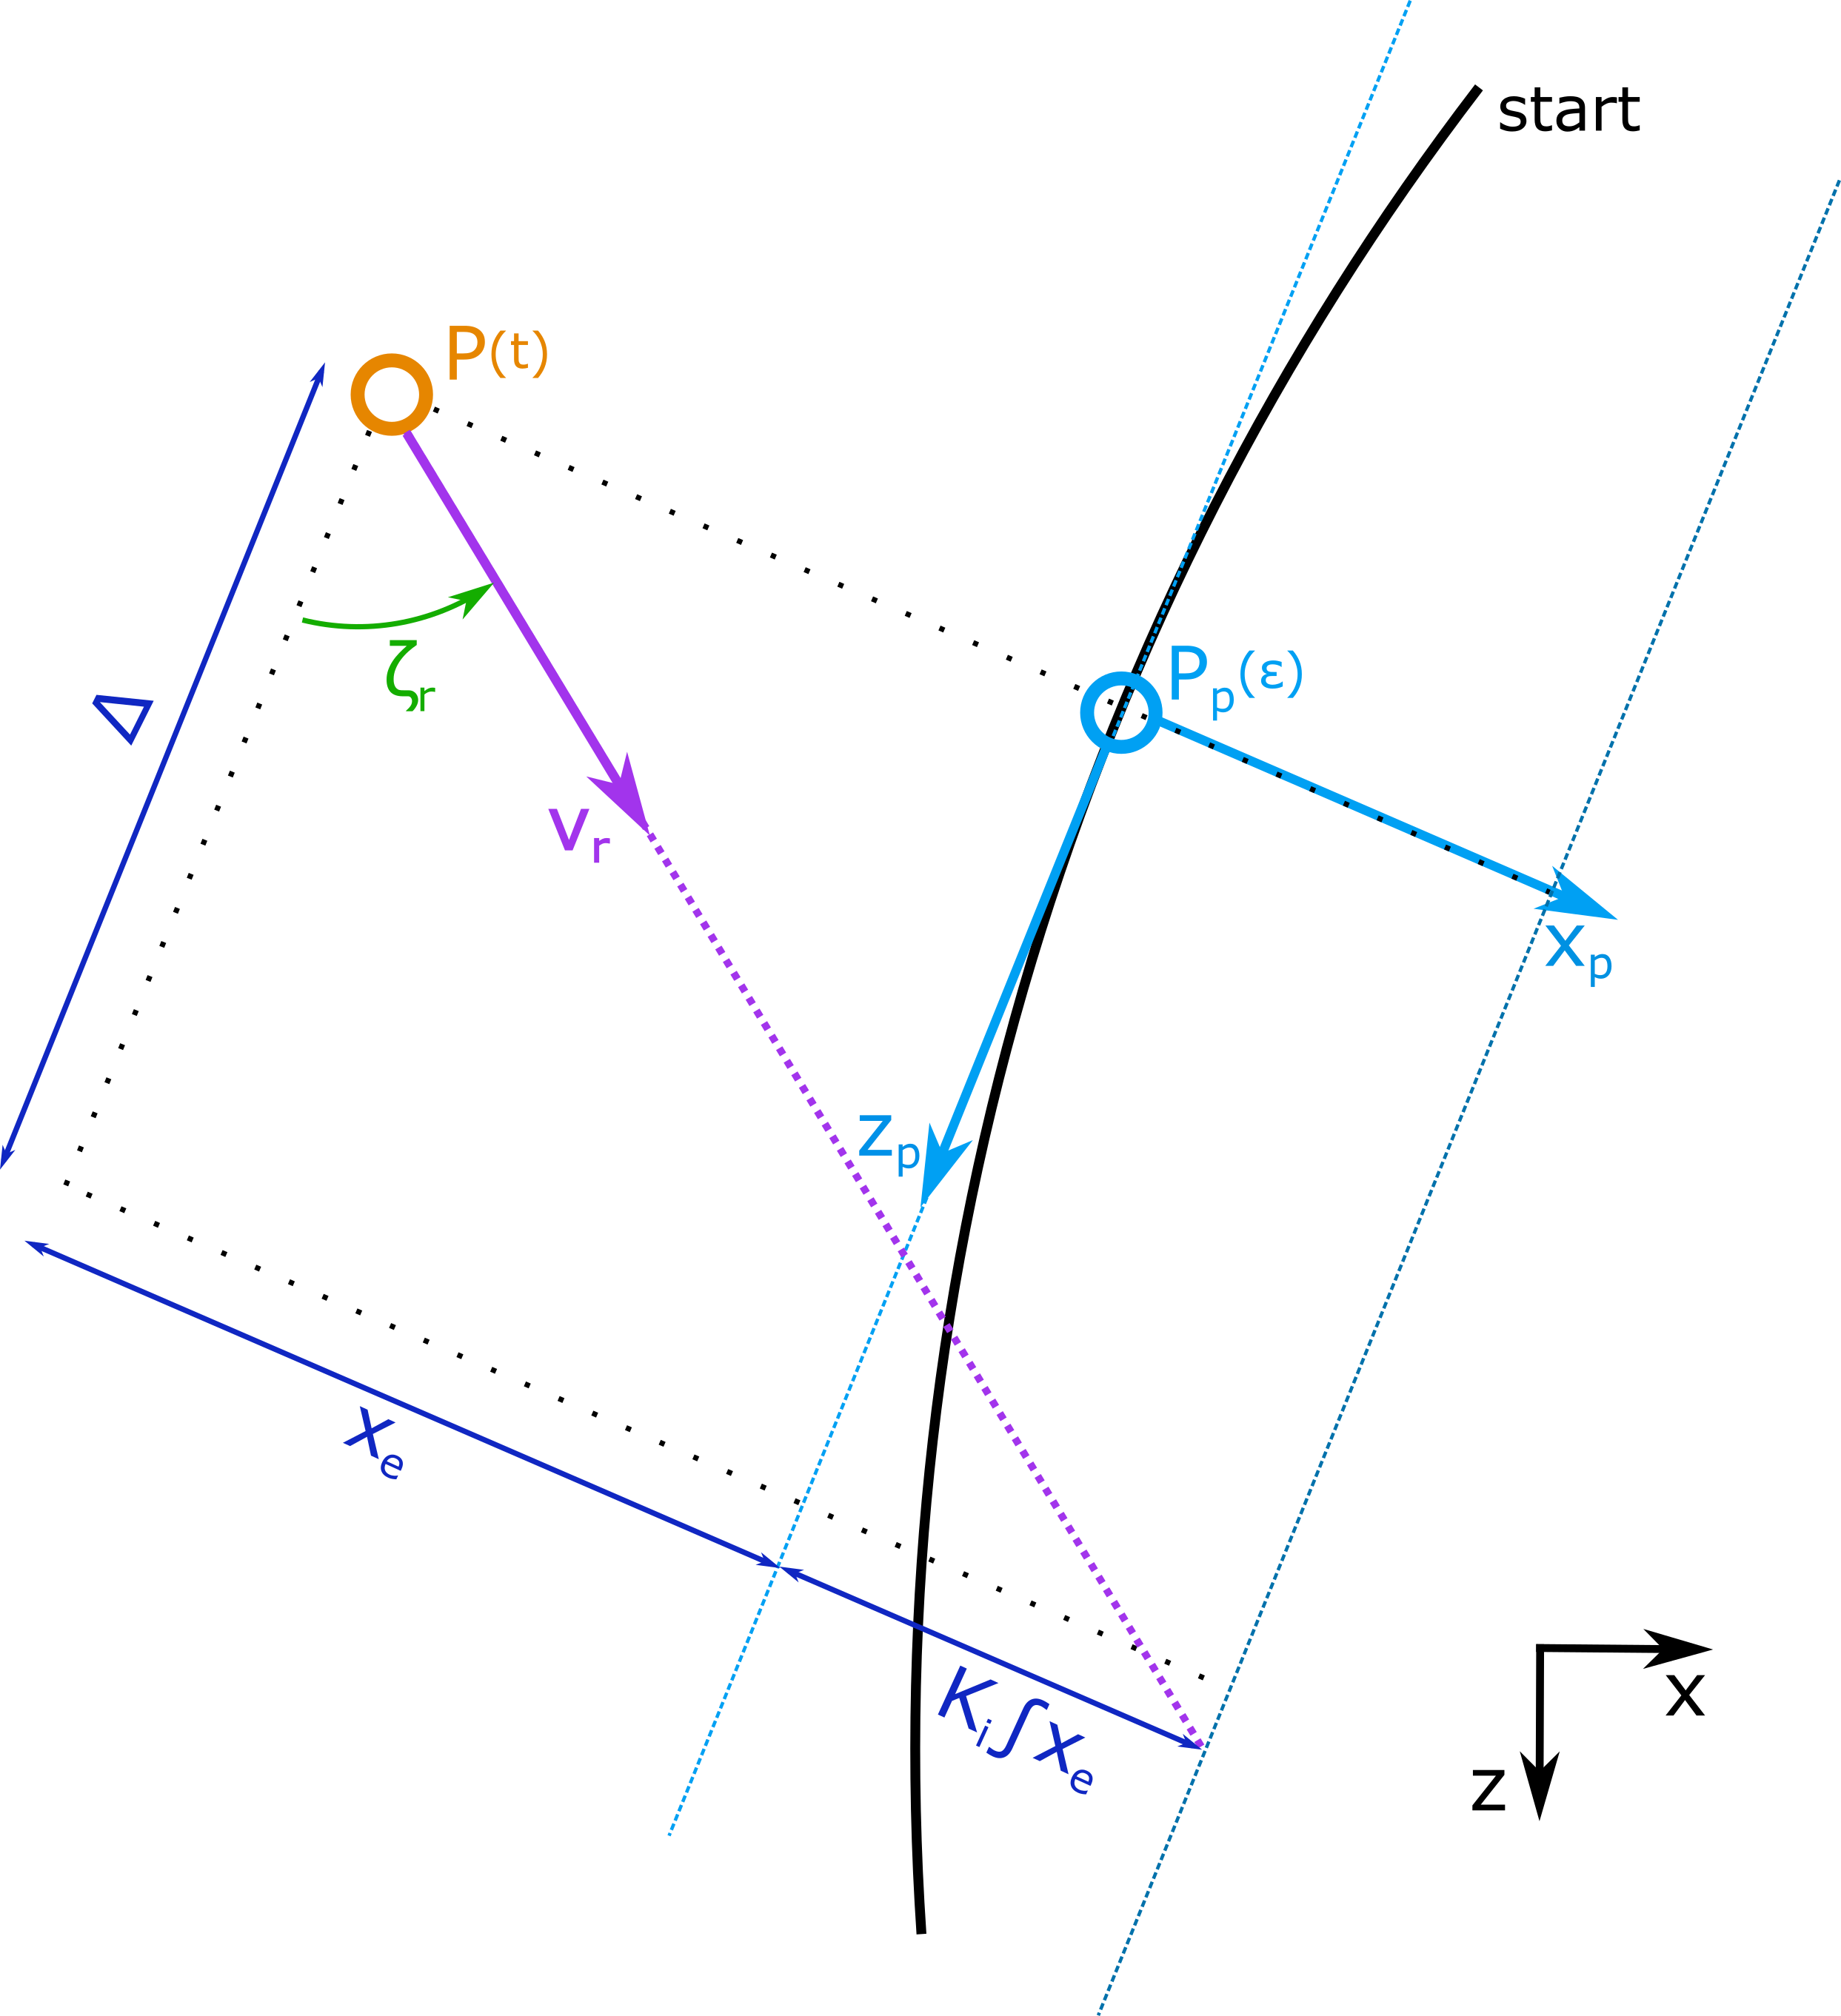
\includegraphics[width=0.65\linewidth]{images/inkscape/ILOS.png}
    \caption{Visualization of the variables associated with ILOS steering for curved paths}
    \label{fig:ilos}
\end{figure}

And the reference steering angle \(\theta_r\) with ILOS guidance remains identical to equation (28), only with a re-definition of the \(\zeta_r\) parameter.

\subsubsection{Ribbon Adaptation Motivation and Design}
A later addition to the design of the system is the ribbon adaptation module. This module is responsible for taking in the desired curvature and giving out the desired device-specific actuation \(u_d\) needed for this device to achieve the desired curvature. 

\paragraph*{Ribbon Adaptation Motivation}
During testing it was observed that devices would display markedly different dynamics, but also the same device could behave differently from day to day. This is likely due to wear in terms of gelatin from the brain phantom entering the ribbon and hardening inside the tendon tracks leading to higher internal friction over time (more on this in the results section). Although a small difference from day to day was also observed when the device had not been inserted into gelatin. An example of of the inter-day differences can be seen when comparing figure \ref{fig:scaledaxis} to \ref{fig:bigamp}. 
\newline \newline 
These plots show the acquired curvature (in air) when a certain tendon actuation is applied (more on how this is done in the methods chapter on ribbon adaptation). These two plots show the behavior of the same ribbon, but some days apart. As we can see the curvatures achievable by the ribbon in figure \ref{fig:bigamp} are approximately double the curvatures achieved the ribbon in figure \ref{fig:scaledaxis} at the same tendon actuation. 

\begin{figure}[H]
    \centering
    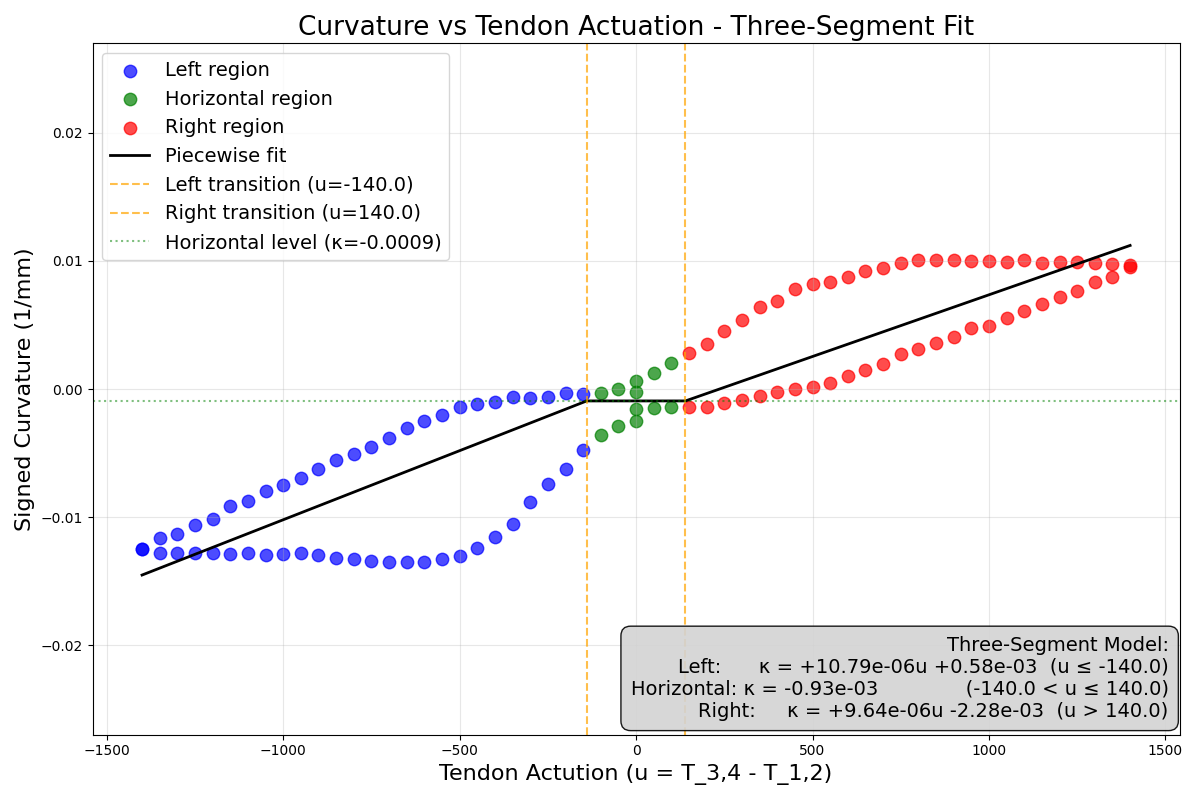
\includegraphics[width=0.9\linewidth]{images/ribbonadapter/Ribbonfit_2025-06-27_18-55-42-scaledaxis.png}
    \caption{Measured curvature of the ribbon in air as a function of tendon actuation. The ribbon shows limited curvature response compared to figure \ref{fig:bigamp}}
    \label{fig:scaledaxis}
\end{figure}

\begin{figure} [H]
    \centering
    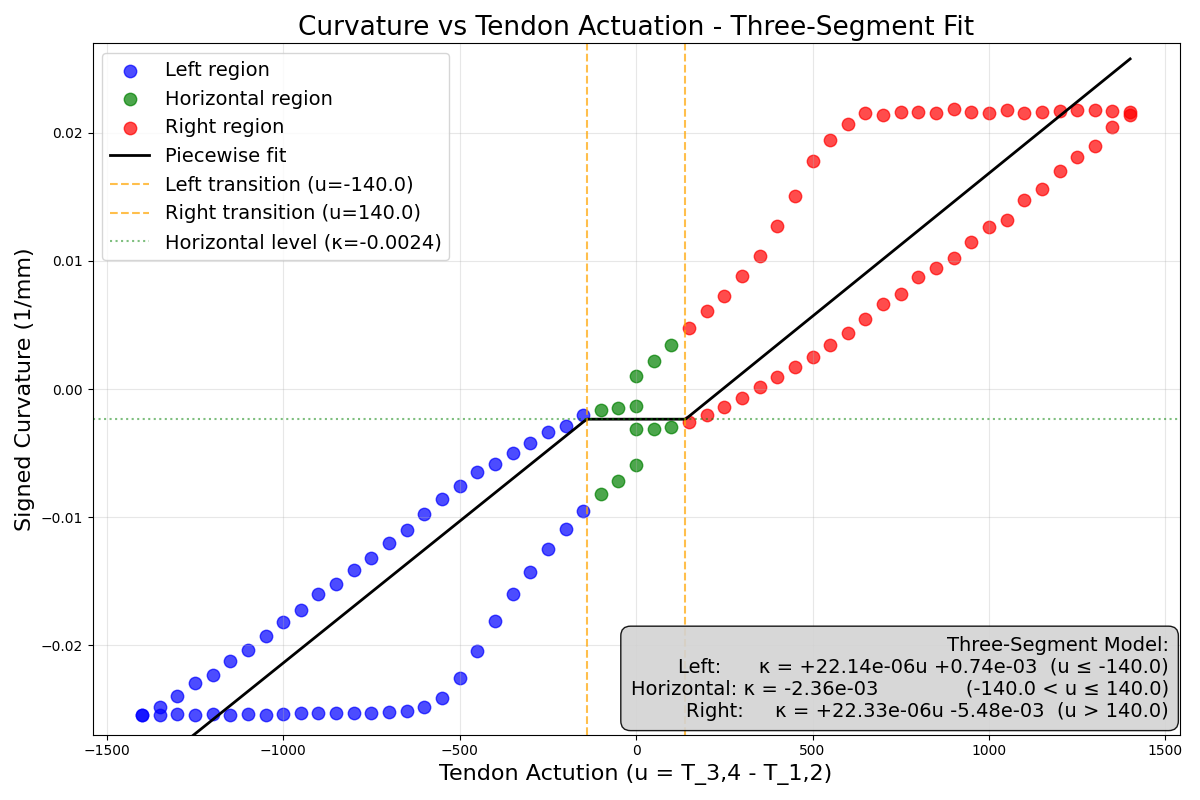
\includegraphics[width=0.9\linewidth]{images/ribbonadapter/RibbonFit_2025-07-03_09-38-33.png}
    \caption{Measured curvature of the same ribbon in air at the same tendon actuation range. Curvature amplitudes are roughly double those seen in Figure \ref{fig:scaledaxis}, indicating reduced internal friction.}
    \label{fig:bigamp}
\end{figure}

If one were not to take into account this difference in behavior and would simply output the same desired tendon actuation, \(u_d\), on every day for every device the system would work very poorly. Particularly PI feedback controller that ensures that the measured pitch \(\theta_m\) tracks the desired pitch \(\theta_r\) would be impossible to tune as the same control gains could lead to either sluggish under performance or unstable overshooting. This variability would severely degrade tracking accuracy and result in very little reproducibility and require re-tuning for every day. It was therefore decided that it was necessary to implement some way of taking this day-to-day and device-to-device variability into account.

\paragraph*{Ribbon Adaptation Design }
In order to implement the adaptation strategy several options were considered. Since an autopilot for the pitch had already been designed and implemented (before the extent of the variability was understood) the first evaluated approach was to automatically tune the existing PI controller for the pitch. Several analogous cases for ships were found including \cite{puntunan_online_2006}, \cite{tomera_fuzzy_2017}, \cite{zhang_-line_2020}, \cite{tung_self-tuning_2023} where self-tuning PID controllers were implemented using methods such as fuzzy logic and neural networks. However, these approaches were all quite complex and more importantly required extensive data for proper tuning. For the the ribbon system, collecting this amount of data would have required numerous runs in gelatin. This presented a major issue since running the ribbon in gelatin before surgical use would risk risk contamination making it unsuitable for insertion after tuning. 
\newline \newline
Therefore a completely different approach to the problem was taken. Instead of adaptively tuning the pitch PI controller, the output of the controller would be adapted to each device. This meant that instead of the PI controller directly outputting the desired tendon actuation, it would output a desired curvature. This curvature would then be converted into the appropriate tendon actuation based on the dynamics of that specific device.
\newline \newline
Several methods of identifying this mapping between the curvature and tendon actuation were evaluated. The most accurate approach would have involved running a full length insertion into gelatin at various constant tendon tensions and then identifying the resulting curvatures. However this would have required a lot of time and would pose the same issue as previously: contaminating the device. Therefore a much less time consuming approach of observing the resulting curvatures of different tensions in air was chosen. This still results in conversion equations specific for each device, and as it was expected that as long as the PI control was  tuned based on this air conversion the difference in medium would have minimal impact on control performance.

\lhead{2D Path following - Methods} % section header
\subsection{Methods}

\subsubsection{Path-Following Implementation Methodology}
In order to ensure that later expansions or improvements to the 2D path-following would be easy to implement and the system be highly readable the  system is implemented using a modular architecture that consists of a \texttt{GuidanceSystem}, \texttt{PitchConverter}, \texttt{FeedbackController}, \texttt{FeedforwardCalculator}, \texttt{RibbonAdapter} and \texttt{TensionConverter}. These modules correspond to classes in the code base inside the pathfollowing folder and correspond directly to the modules in the control system diagram as can be seen in figure \ref{fig:2DpathfollowingSystemControlDiag}. 

\begin{figure} [H]
    \centering
    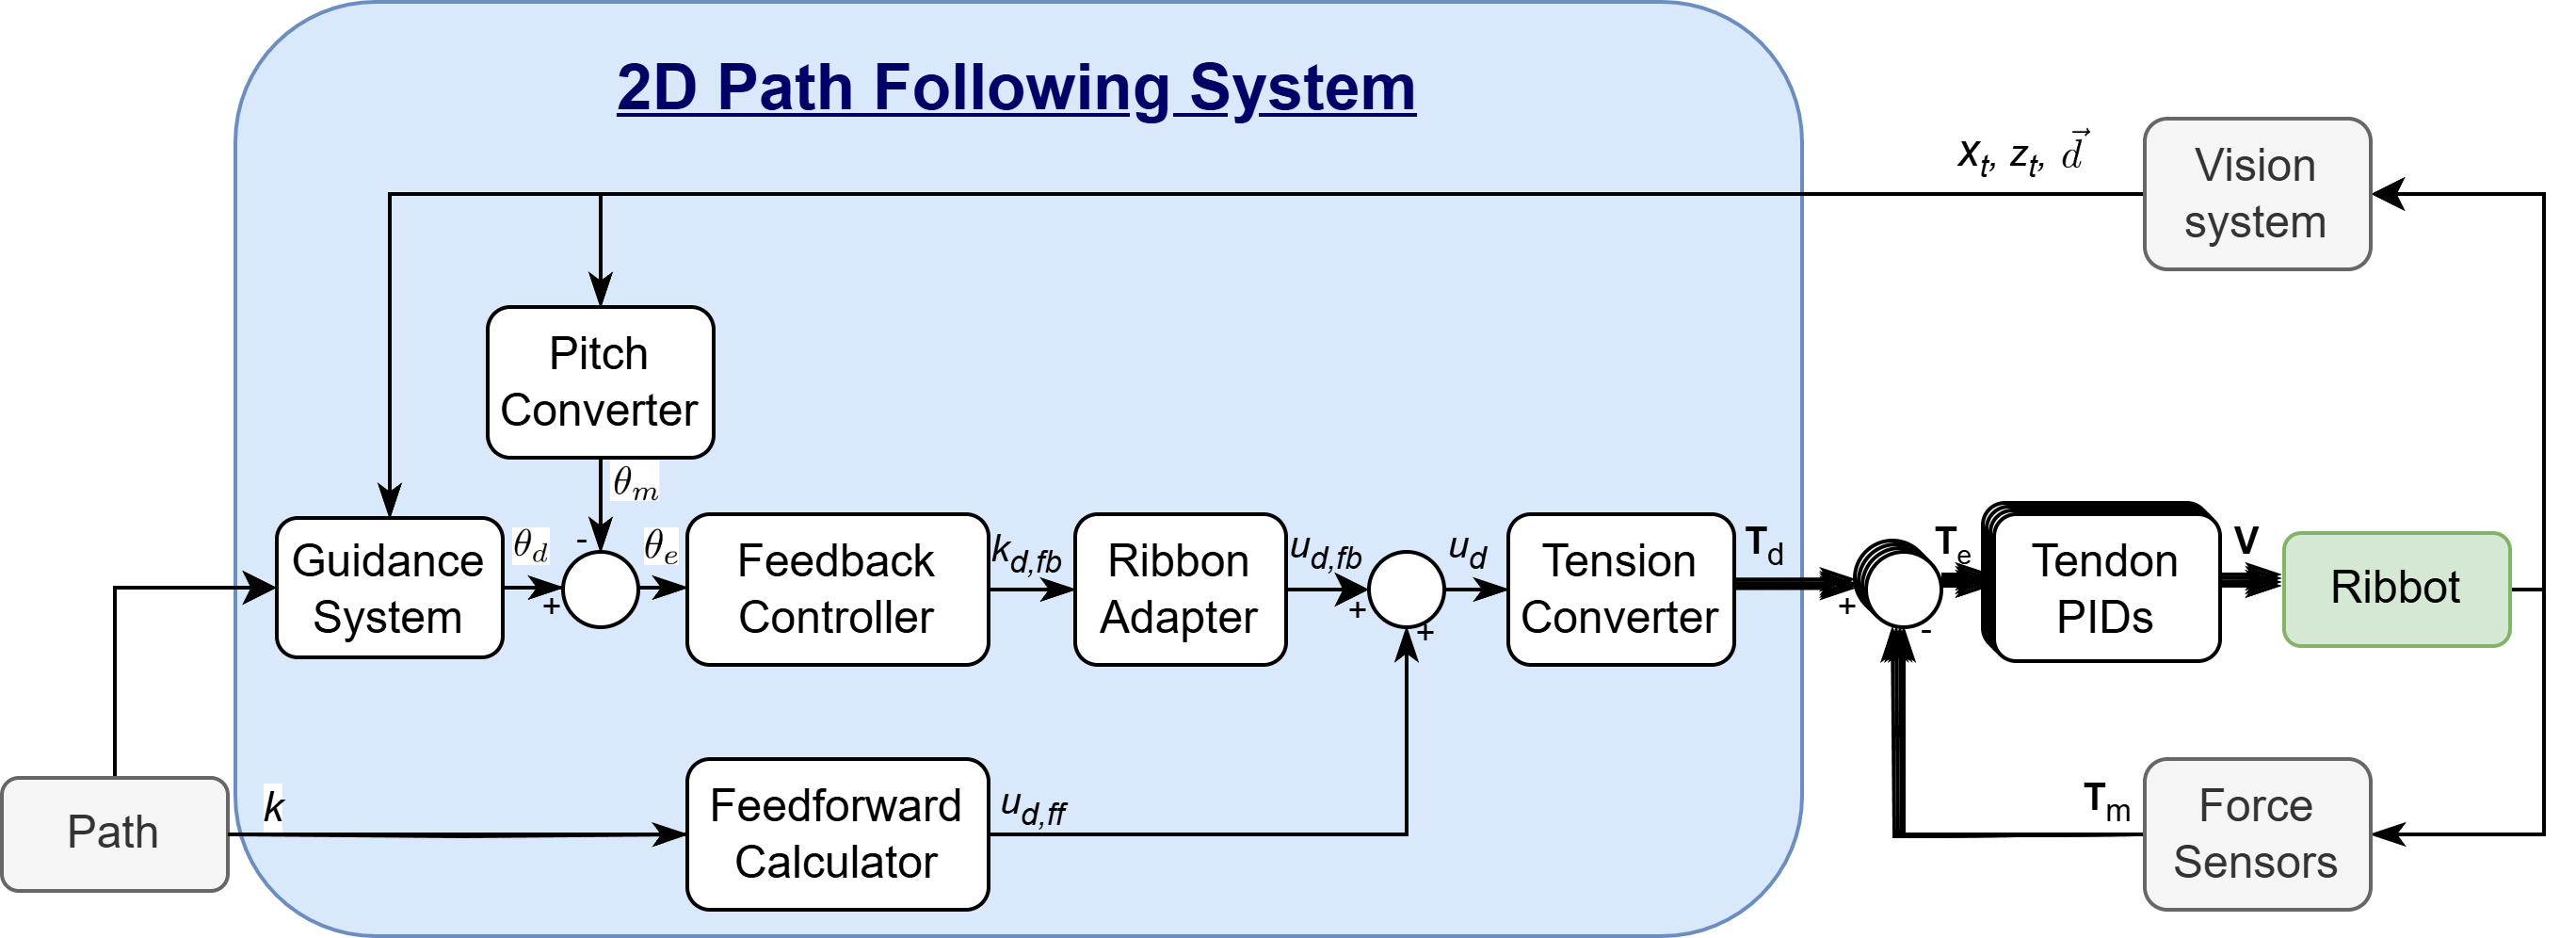
\includegraphics[width=\linewidth]{images/RibbotControl_2Dpathfollowing400p.png}
    \caption{Visualization of the 2D path following system section of the full control system}
    \label{fig:2DpathfollowingSystemControlDiag}
\end{figure}

In order to orchestrate the cooperation between these classes and their dataflow the \texttt{PathFollower} class was created. This class is also responsible for communicating with the rest of the code base. Its connection to the other classes can be seen in figure \ref{fig:pathfolloingmodules}.   In the later chapter on implementation each of the modules are expanded upon and explained.

\begin{figure}[H]
    \centering
    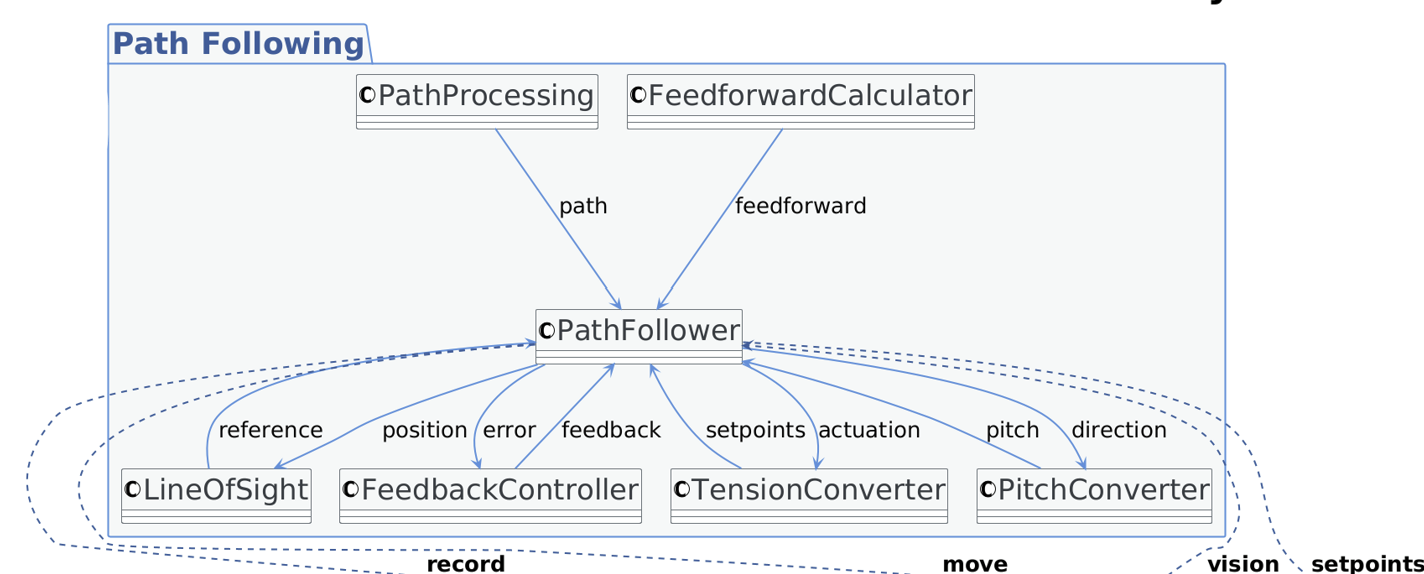
\includegraphics[width=\linewidth]{images/Software documentation/pathfollowingmodules.png}
    \caption{Path following system architecture}
    \label{fig:pathfolloingmodules}
\end{figure}

\subsubsection{Ribbon Dynamics Identification Process}
This subsection describes the methodology behind identifying the device specific curvature vs tendon actuation conversion equations necessary for the ribbon adaptation described in the design chapter. The process consists of four steps which are described below in the  order of execution.

\paragraph*{Applying the Tendon Actuation Values}
The first step is to start the vision system and then press the start calibration button in the GUI. This triggers a method in the \texttt{AirCalibrator} class that begins by pushing the ribbon out of the feeder by 40mm, and then begins a sequence of applying increasing tensions on one side from 100mN up to 1500mN, in 50mN intervals, sending a command to the python program to capture a picture such as the one in figure \ref{fig:pictureRibbon} at each actuation setpoint. After reaching 1500mN it steps the tension down again using the same intervals until the tension on all tendons is neutral i.e. 100mN. Thereafter it repeats the same process on the other side. Finally it retracts the ribbon back to its original position.

\paragraph*{Extracting the Resulting Curvatures}
In order to determine the resulting curvatures at each tension actuation value the \texttt{curvaturedetector.py} script was written. This script processes each image captured during calibration by first subtracting the background (an image captured automatically before moving the ribbon) and skeletonizing the difference to extract the ribbon's centerline. The extracted centerline is then down sampled to fit a smooth spline, and the curvature is estimated by fitting a circle to the spline points and computing its signed curvature. It optionally generates visual debug images showing the detected centerline and the fitted circle such as the one in figure \ref{fig:centerline} The script also automatically matches each image with its corresponding tension value (extracted from the metadata in the filename), and saves the resulting curvatures in a CSV file.

\begin{figure}[H]
    \centering
    \begin{subcaptionbox}{Picture taken by the python vision program at a tendon actuation of +1500mN, such pictures are taken at 50mN intervals for later use in curvature detection \label{fig:pictureRibbon}}[0.45\linewidth]
        {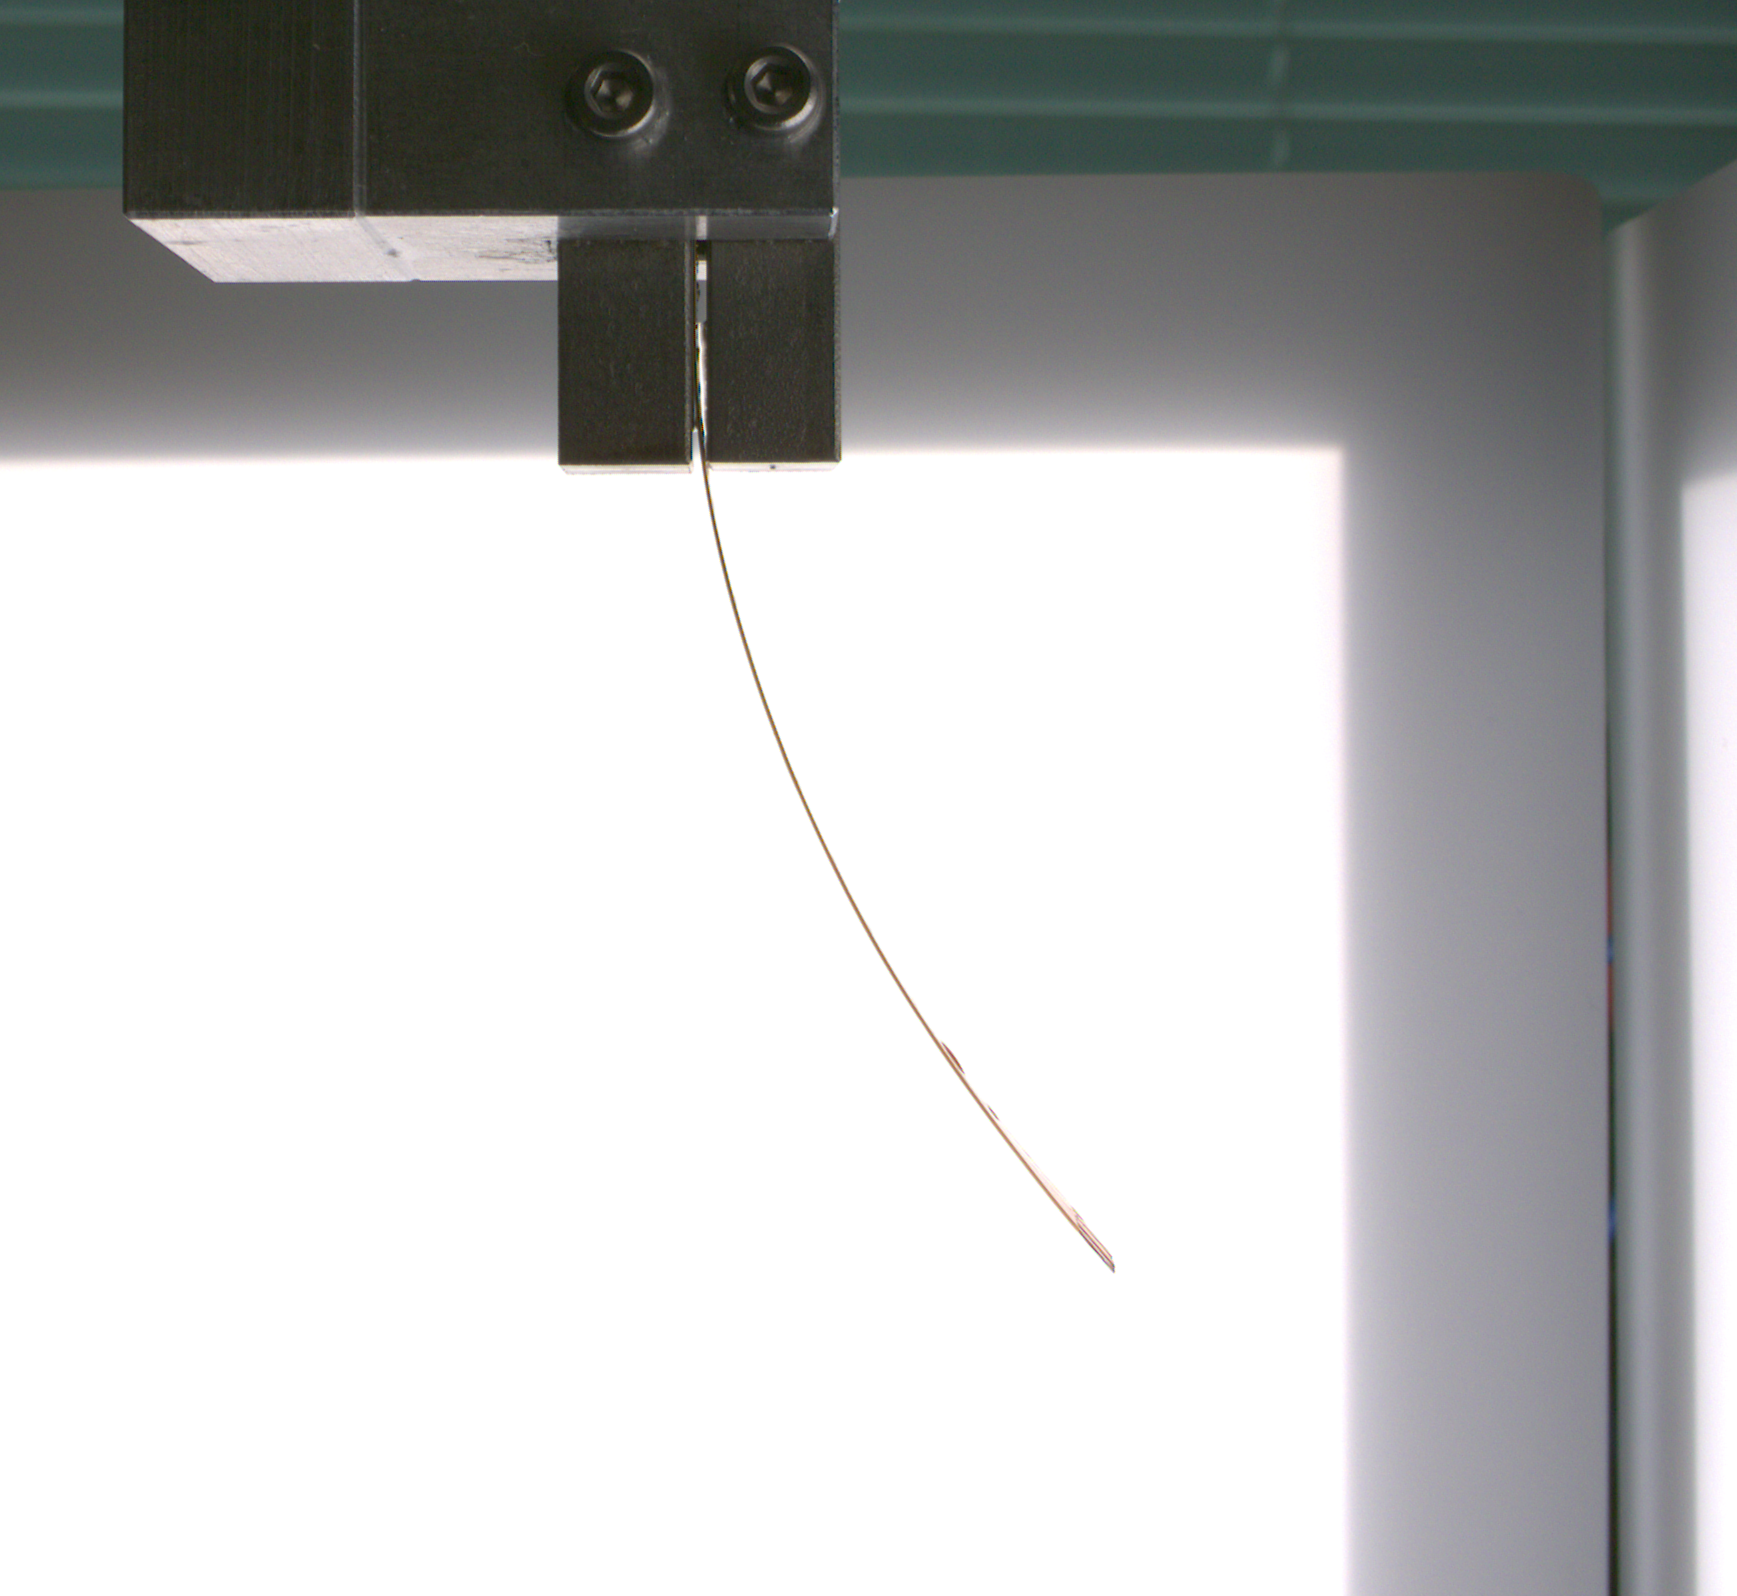
\includegraphics[width=\linewidth]{images/ribbonadapter/aircalib_right_tension1500_2025-06-17_17-36-39_cam23.png}}
    \end{subcaptionbox}
    \hspace{0.05\linewidth}
    \begin{subcaptionbox}{Visual debug image generated for (a) by the \texttt{curvaturedetector.py} script, such images are created for every corresponding image taken during the calibration process, visualizing the detected centerline as well as the fitted circle \label{fig:centerline}}[0.45\linewidth]
        {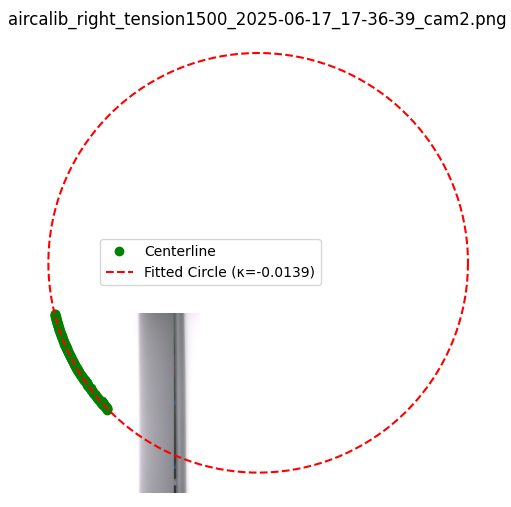
\includegraphics[width=\linewidth]{images/ribbonadapter/aircalib_right_tension1500_2025-06-17_17-36-39_cam2_debug3.png}}
    \end{subcaptionbox}
    \caption{Tendon calibration procedure and resulting curvature extraction. (a) Raw image captured at a tendon actuation of 1500mN during the calibration routine. (b) Corresponding debug output generated for determining resulting curvature.}
    \label{fig:ribbonadaptation}
\end{figure}

\paragraph*{Fitting the Curvature-Tension Function}
Then to determine the conversion function from tendon actuation to curvature another script \texttt{curvatureVsTnsion.py} was written. It reads the curvature results, assigns signed tension values based on whether the left or right tendons were actuated, and fits a continuous piecewise function with three segments: a linear slope for left actuation, a flat horizontal segment around zero tension representing the ribbon’s pre-curvature at neutral tension and its deadzone, and a second linear slope for right actuation.
\begin{figure} [H]
    \centering
    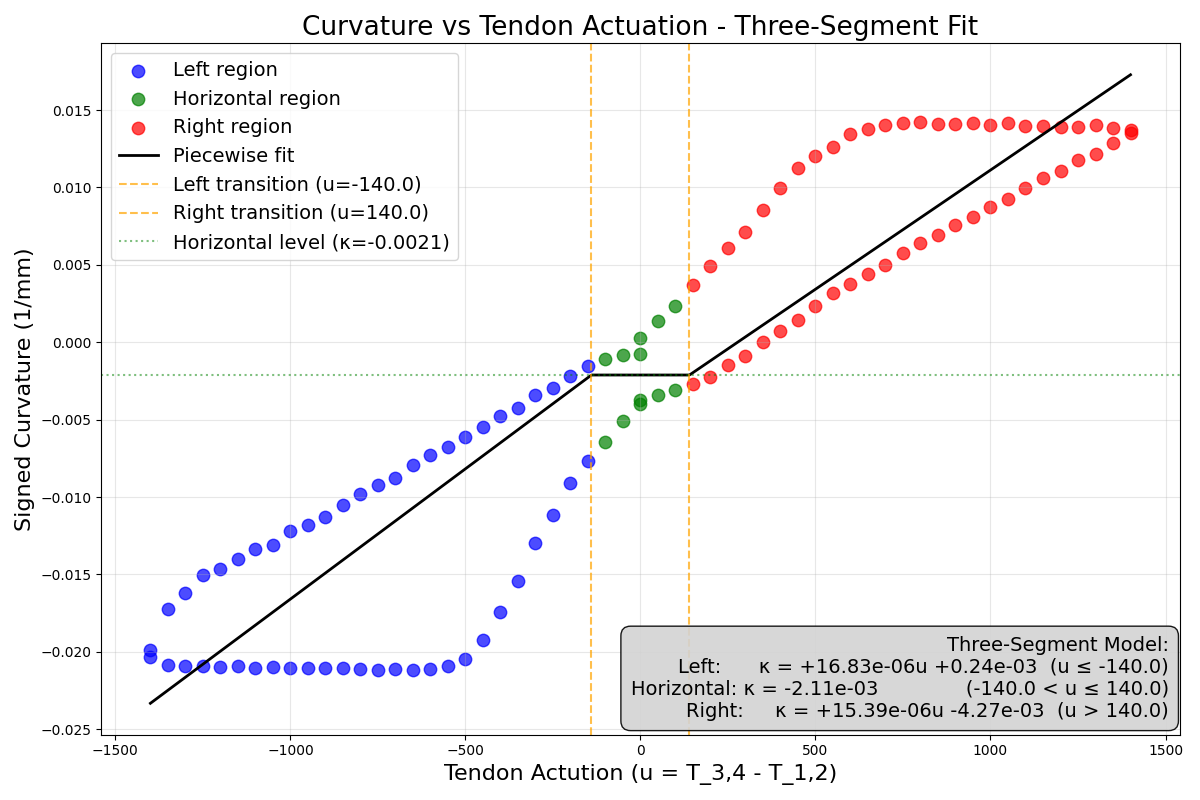
\includegraphics[width=0.9\linewidth]{images/ribbonadapter/ribbonfit_2025-06-30_15-59-06.png}
    \caption{Result of running the \texttt{curvatureVsTension.py} script which fits a three segment model by optimization to relate Curvature and Tendon actuation}
    \label{fig:curvaturevstension}
\end{figure}
The script uses a weighted least-squares optimization to emphasize the accuracy of the horizontal segment since that has less data point than the other segments, and allows for asymmetry between the left and right sides. To find a good fit, the script uses a multi-start approach where it generates a wide range of initial uesses for the segment voundaries and slope parameters. Each candidate is optimized using the Sequential Leas Squares Programming (SLSQP) method provided in by the \texttt{Scipy minimize} method. The best-performing model is selected based on the lowest weighted error. The final function is then plotted along with the expression for each segment (as seen in figure \ref{fig:curvaturevstension} which are later used in the control system.

\subsection{Feedforward Characterization Process}
\todo{write section?}

%\subsubsection{Tuning Methodology}
%\todo{write section?}

%\subsubsection{Validation Plan for Path-Following}
%\todo{write section?}


\lhead{2D Path following - Implementation} % section header
\subsection{Implementation}
This subsection briefly describes how every module in the path following part of the control system visualized in figure \ref{fig:2DpathfollowingSystemControlDiag} is implemented in the code base. 

\subsubsection{Guidance System (LOS and ILOS)}
The guidance system module responsible for taking in the path and outputting the reference pitch angle \(\theta_r\) was implemented in two different ways. First a classic LOS module was implemented, then later in the thesis this was switched out with an ILOS guidance system.
\paragraph*{Line-Of-Sight (LOS)}
The LOS system design described earlier is discretized and implemented in the \texttt{LineOfSight} class and is responsible for calculating \(\theta_r\) based on the probe's current tip position and a set of predefined waypoints. The closes point on the path is selected by minimizing the Euclidean distance between the tip and all path points
\begin{equation}
\epsilon^* = \arg\min_\epsilon \left\{ (x - x_\epsilon)^2 + (z - z_\epsilon)^2 \right\}
\end{equation}
From the selected path point \(P_p(\epsilon) = [x_\epsilon, z_\epsilon]^T\), the path tangential angle is computes as 
\begin{equation}
\zeta_p = \arctan\left(\frac{x_\epsilon - x_{\epsilon-1}}{z_\epsilon - z_{\epsilon-1}}\right)
\end{equation}
Then the corss-track error is calculated by projecting the positional error onto the normal of the path
\begin{equation}
    x_e = (x - x_\epsilon)\cos\zeta_p - (z - z_\epsilon)\sin\zeta_p
\end{equation}
Finally the LOS steering correction is calculated according the LOS steering law 
\begin{equation}
    \theta_r = \zeta_p + \arctan\left(\frac{-x_e}{\Delta}\right)
\end{equation}
This pitch angle is updated each time new tip coordinates are received from the vision system and passed to the pitch autopilot for control.


\paragraph*{Integral-Line-Of-Sight (ILOS)}
To improve robustness against steady-state path following errors, and ILOS extension of the LOS was implemented in the same \texttt{LineOfSight} class. The ILOs method uses the same core logic as LOS for computing the tangential path angle \(\zeta_p\) and cross-track error \(x_e\), but integrates the cross-track error over time to form an additional correction term. On each call, the integration is updated as:
This integral term is updated in discrete time based on the elapsed time \(\Delta t\) between two consecutive calls:
\begin{equation}
x_{e,\text{int}}[k] = x_{e,\text{int}}[k-1] + x_e[k] \cdot \Delta t
\end{equation}
To ensure numerical stability, this accumulated error is clamped between predefined bounds:
\begin{equation}
x_{e,\text{int}}[k] = \text{clamp}\left(x_{e,\text{int}}[k], x_{\text{min}}, x_{\text{max}}\right)
\end{equation}
The final pitch reference angle is then computed using the ILOS steering law:
\begin{equation}
    \theta_r = \zeta_p + \arctan\left(\frac{-x_e - K_i \cdot x_{e,\text{int}}}{\Delta}\right)
\end{equation}
Where the integral gain \(K_i\) is a design parameter.

\subsubsection{Pitch converter}
The pitch autopilot is a closed-loop control system that continuously regulates the pitch of the tip. The autopilot layer consists of three primary components: a pitch angle converter, a feedback controller, and a tension converter. Together, these components transform the LOS heading reference into actuator-level tendon tension setpoints.

The first step in the autopilot is estimating the measured pitch angle, \(\theta_{meas}\), from vision data. This is simply done by computing the angle between the z-axis and the 3D direction vector defined by the detected tip and pre-tip positions. 
\begin{equation}
    \theta_{meas} = atan2(\vec{d}_x,\vec{d}_z)
\end{equation}
where \(\vec{d}_x\) and \(\vec{d}_z\) are the \(x\)- and \(z\)- components of the direction vector. This computation is implemented in the \texttt{PitchConverter} class.

\subsubsection{Feedback controller}
The main component of the pitch autopilot is the PI controller implemented in the \texttt{FeedbackController} class. The controller receives the pitch error, defined as 
\begin{equation}
    \theta_e = \theta_{ref} - \theta_{meas}
\end{equation}
and calculates a curvature command \(\kappa_{d,fb}\) intended to minimize the error. 
\newline \newline 
A curvature control output is natural here as the ribbon changes direction based on the bending of the distal segment. This bending does not directly set the orientation of the tip but instead defines the spatial rate of change of the orientation, that is, the curvature of the path followed by the tip. The curvature determines how the pitch angle evolves as the probe advances. Since the device moves at a constant speed the curvature can also be understood as the rate of change of the pitch angle \(\theta_m\), making it a useful control variable.
\newline \newline
Since the ribbon system is highly damped, derivative control is unnecessary and therefore a PI controller was implemented with anti-windup for the integral term.
\begin{equation}
    \kappa_{d,fb}(t) = K_p \theta_e(t) + K_i \int \theta_e(t)
\end{equation}
Since the pitch control loop is triggered asynchronously by new vision data and the arrival time fo these updates may vary, the effective sampling time \(\Deltat\) is computed each time using system timestamps. This ensures the validity of the integral terms.

\subsubsection{Feedforward Calculator}
There is also a feedforward component that provides open-loop commands to follow the curvatures in the desired path geometry. This is implemented in the \texttt{FeedforwardCalculator} class, which pre-computes actuation commands for each waypoint along the planned trajectory. 

The \texttt{FeedforwardCalculator} processes the entire planned path to generate a lookup table of actuations indexed by waypoint position. This lookup table is based on previous characterization experiments that established the mapping between required tendon tension and achieved curvature. However, since the path generator creates trajectories consisting of discrete straight and curved segments, directly commanding the ideal tension for each segment would create large instantaneous changes that the physical tendon system cannot follow.

To address this limitation, the feedforward controller implements a ramping strategy between segments. The ramp length is calculated based on the magnitude of the required actuation change and the known response capabilities of the tendon system:

\begin{equation}
\text{rampLength} = \frac{\text{setpointRampRate} \cdot v_{target} \cdot 1000}{|\kappa_{d,ff}(i+1) - \kappa_{d,ff}(i)|}
\end{equation}

The ramping region spans the end of the current segment and the beginning of the next segment, with the actuation linearly interpolated between the ideal values for each curvature. This approach allows the tendon system sufficient time and distance to transition smoothly between the required tensions for different path curvatures, ensuring that the feedforward commands remain physically realizable by the actuation hardware.


\subsubsection{Ribbon Adapter}
The \texttt{RibbonAdapter} module translates desired curvature commands from the feedback controller into the appropriate control variable \(u_{d,fb}\) for the specific ribbon device. This adaptation accounts for the individual curvature-tension characteristics of each ribbon. This conversion is based on the ribbon dynamics identification process described in the methods section, which establishes the relationship between applied tendon actuation and resulting tip curvature for the given ribbon. As shown in figure \ref{fig:curvaturevstension}, the relationship is modeled as a three-segment piecwise funciton consisting of a central horizontal region (the pre-curvature deadzone) and two linear slopes for left and right bending. These parameters in the bottom right fhese functions are entered into the system via the calibrator tab in the GUI \ref{fig:calibratortab}
\begin{figure}
    \centering
    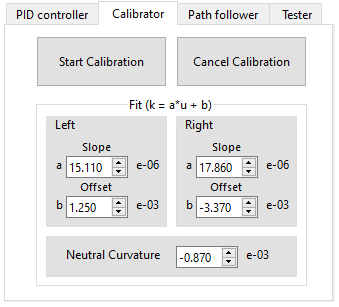
\includegraphics[width=0.5\linewidth]{images/gui/calibrator.PNG}
    \caption{Calibrator tab where the user inserts the ribbon dynamics identified by running the ribbon dynamics identification process}
    \label{fig:calibratortab}
\end{figure}

In the implementation, the adapter selects either the left or right slope and offset depending on whether the desire curvature is above or below the ribbon's neutral pre-curvature. The actuation value is then computed using the following expression:
\begin{equation}
u = \frac{|\kappa_{output}| - \text{Offset}}{\text{Slope}}
\end{equation}
Then the controlvariable is given the same sign as the curvature to maintain the correct bending direction, with positive values corresponding to rightward deflection and negative values to leftward deflection.
\newline \newline
The output of the controller is a scalar actuation variable \(u_{d,fb}\) that represents the differential tension required between the left and right tendon groups. This value is later converted into explicit tendon tension setpoints in the next stage of the pitch autopilot.

\subsubsection{Tension converter}
The final step in the control loop is converting the actuation variable that is defined as 
\begin{equation}
    u(t) = T_{3, 4} - T_{2,1}
\end{equation}
Where \(T_{3, 4}\) and \(T_{1, 2}\) signify the tension on tendons 3 and 4 on the right and 1 and 2 on the left respectively.

The conversion stage maps the scalar actuation variable to individual tendon tensions, while maintaining a baseline tension of 100mN on all tendons to prevent slack. The conversion logic is:
\begin{equation}
\begin{cases}
T_1 = T_2 = 100 \text{ mN}, \quad T_3 = T_4 = 100 + u & \text{if } u > 0 \
T_1 = T_2 = 100 + |u|, \quad T_3 = T_4 = 100 \text{ mN} & \text{if } u < 0 \
T_1 = T_2 = T_3 = T_4 = 100 \text{ mN} & \text{if } u = 0
\end{cases}
\end{equation}

The \texttt{TensionConverter} class implements this conversion through the \texttt{convertToTension()} method, which also enforces maximum tension limits to prevent over-actuation that could damage the ribbon.

\subsection{Results}

\subsubsection{Ribbon Adaptation}
After implementing the Ribbon dynamics identification process several interesting observations were made. Two are highlighted here.

\paragraph*{Hysteresis Effect}
Initially the ribbon dynamics identification process was done by stepping up the tension on one side in 50mN intervals, and then after reaching the maximum desired tension it would reset back to neutral tension on all tendons and repeat the process for the opposite side. This resulted in data that appeared highly linear, as can be seen in figure \ref{fig:hysteresis}
\begin{figure} [H]
    \centering
    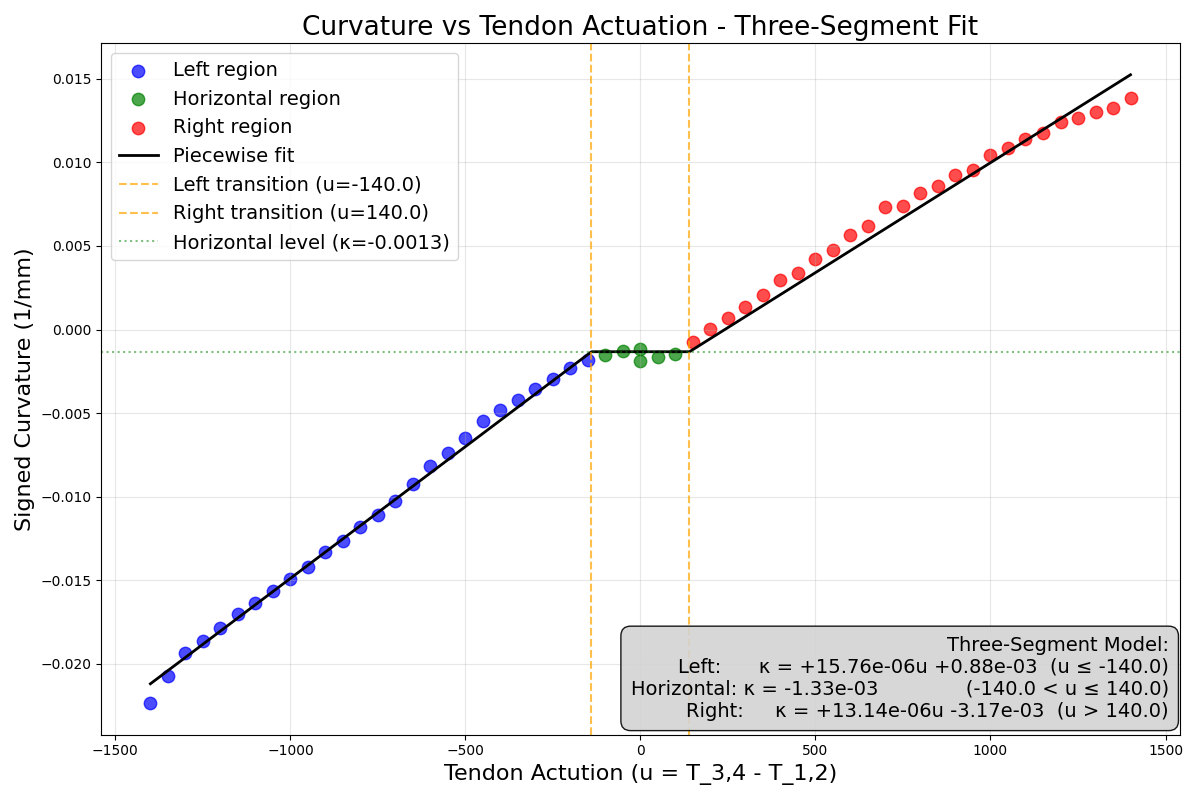
\includegraphics[width=0.9\linewidth]{images/ribbonadapter/Ribbonfit_2025-06-17_17-34-03.png}
    \caption{Initial curvature, tension fit obtained by applying only increasing tensions on each side of the ribbon.}
    \label{fig:hysteresis}
\end{figure}
However during experiments it was observed that the resulting curvature when lowering tension vs increasing tension were different, meaning that there was likely a hysteresis effect. The process was therefore changed to step up the tension and then step it down in order to allow the data to reflect this suspected hysteresis effect. As can be seen in figures \ref{fig:curvaturevstension} and \ref{fig:curvaturevstension2} the hysteresis effect is clearly visible with the curvature not decreasing at all during the initial decreases in tendon tension after having reached the highest tension on each side.


\paragraph*{Effect of Hardened Gelatin}
Another notable effect was the altered ribbon dynamics observed after the ribbon had been inserted into gelatin the previous day. Figure \ref{fig:gelatin} exemplifies the typical response in this state. Paying attention to the values on the y-axis its clear that the ribbon barely curves, even at values as high as 1500mN.
\begin{figure} [H]
    \centering
    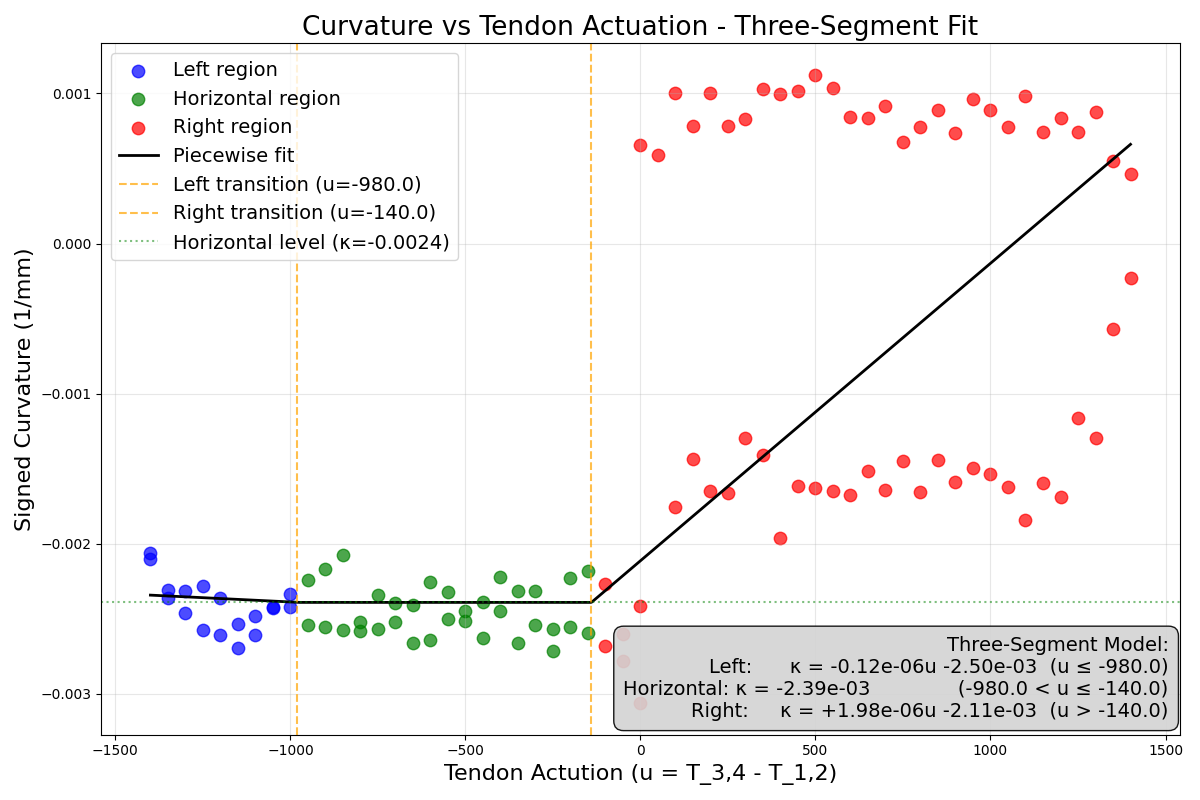
\includegraphics[width=0.9\linewidth]{images/ribbonadapter/ribbonfit_2025-06-27_17-45-46.png}
    \caption{Curvature vs tendon actuation for a ribbon that previously been inserted into gelatin}
    \label{fig:gelatin}
\end{figure}
To address this, the ribbon was cleaned by soaking it in heated, distilled water and pushing out the gelatin in an attempt to dissolve and remove the hardened gelatin. After cleaning, the same ribbon was re-calibrated just 30 minutes later. As shown in figure \ref{fig:curvaturevstension2}, the curvature response returned to expected levels, clearly demonstrating the beneficial effect of cleaning after running experiments in gelatin. 

\begin{figure} [H]
    \centering
    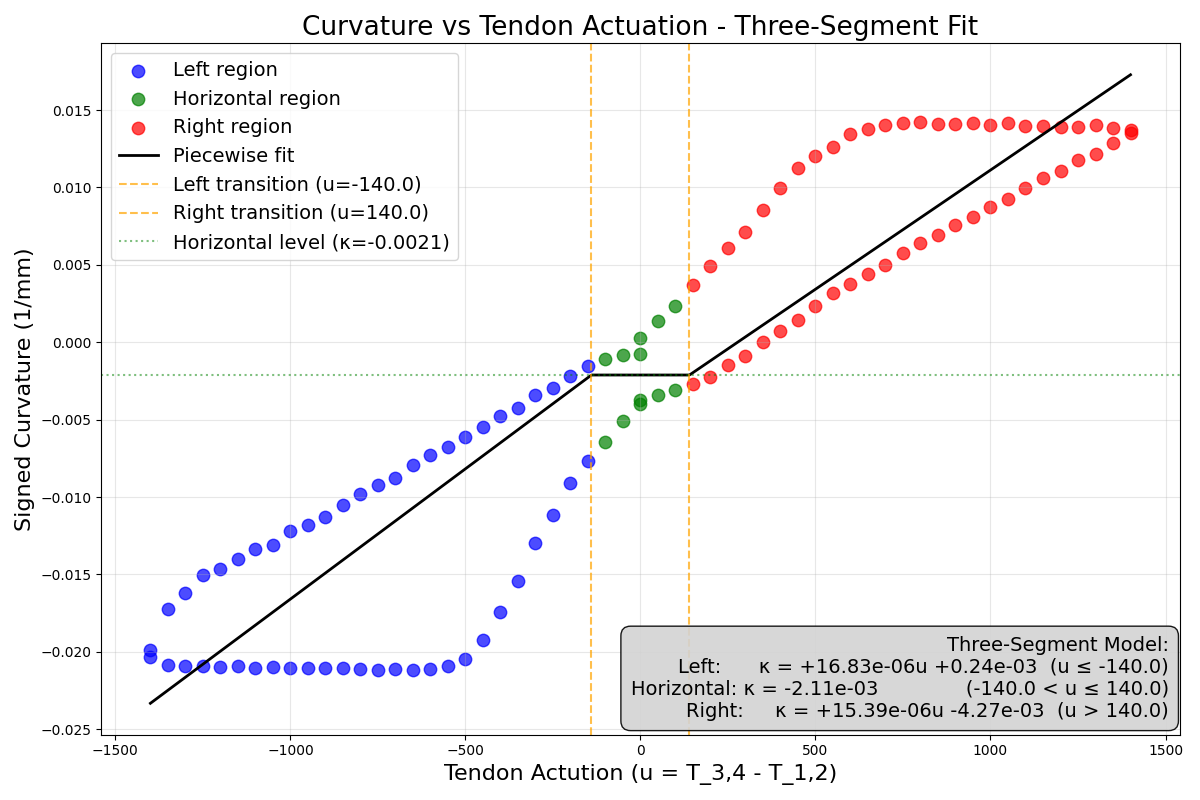
\includegraphics[width=0.9\linewidth]{images/ribbonadapter/ribbonfit_2025-06-30_15-59-06.png}
    \caption{Restored curvature response after cleaning the ribbon.}
    \label{fig:curvaturevstension2}
\end{figure}

\paragraph*{Effect of Dry Tendons}
A similar, yet less severe, degradation in curvature response was observed when the ribbon was completely dry. In this case, the tendons exhibited highly non-linear behavior with limited curvatures, even at high actuation values. This issue was however simply resolved by dipping the ribbon in water prior to calibration. This led to an immediate recovery of the expected curvature-tension behavior.

\subsubsection{Straight Line: Comparing the 3 Guidance Systems}
To compare the performance of the Open-Loop, LOS and ILOS guidance systems, a simplest scenario experiment was made where the ribbon was commanded to follow a straight line through the brain phantom. This controlled scenario was mainly intended to evaluate the system's  tracking accuracy and drift characteristics.

\paragraph*{Open-Loop Straight Line "following"}
Figure \ref{fig:straighol} shows that the open-loop system, which in the case of a straight line applies a constant neutral tension of 100mN on all tendons, fails to maintain accurate path tracking. The error increases steadily over time, a visible drift, with a maximum error of 2.54mm and a mean error of 1.18mm. 
\begin{figure} [H]
    \centering
    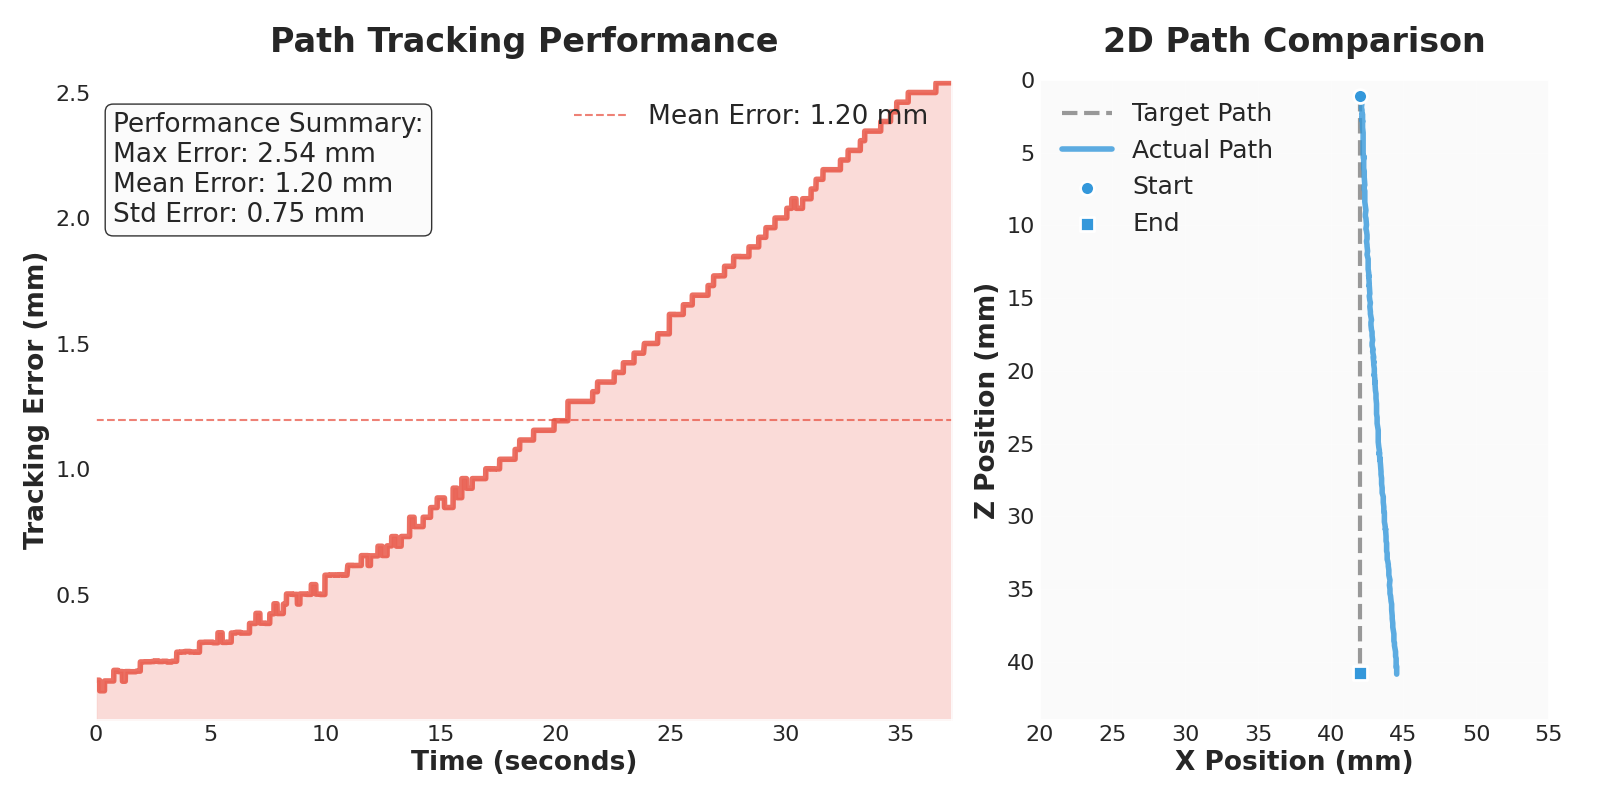
\includegraphics[width=\linewidth]{images/pathfollowing/openloop/straight_20250704_170839.png}
    \caption{Straight line open-loop path "following" performance in a brain phantom}
    \label{fig:straighol}
\end{figure}


\paragraph*{LOS Straight Line Following}
The LOS guidance system demonstrates a significant improvement (see figure \ref{fig:straightLOS})  over the open-loop. The maximum error is reduced to 0.35mm, over 2mm less that the open loop scenario. The mean error is 0.14mm and the tracking error remains relatively stable and low throughout the trajectory. Although a slight increase in error occurs toward the end of the trajectory, the system is able to correct its heading, removing the issue of drift.  
\begin{figure} [H]
    \centering
    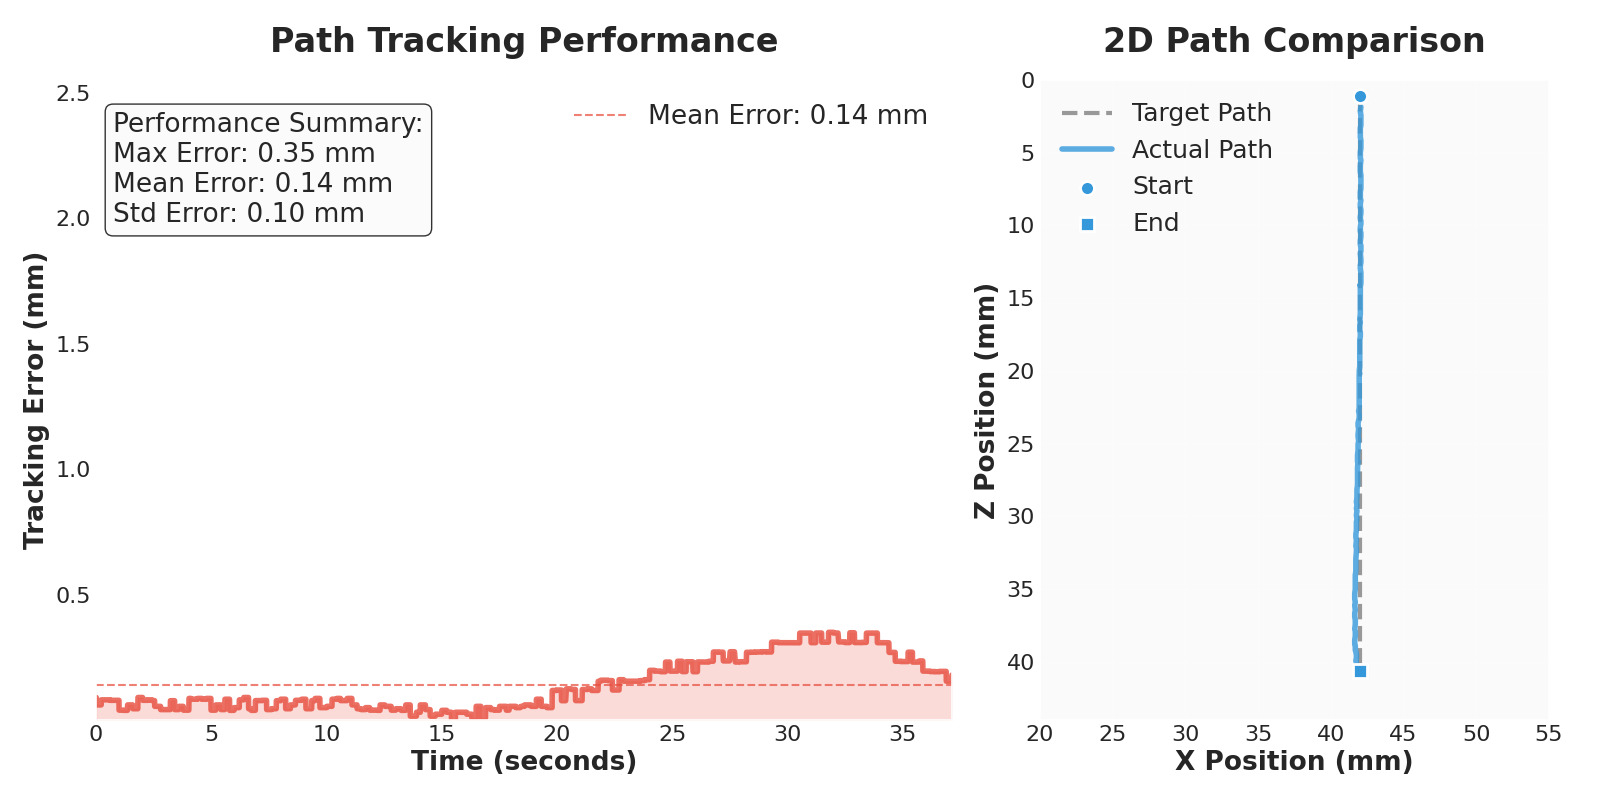
\includegraphics[width=\linewidth]{images/pathfollowing/LOS/straight_250704_164925_scaled.png}
    \caption{Straight line LOS path following performance in a brain phantom}
    \label{fig:straightLOS}
\end{figure}


\paragraph*{ILOS Straight Line Following}
The ILOS controller achieved the highest tracking precision. As seen in figure \ref{fig:straightILOS} the mean tracking error is only 0.08mm with a maximum error of 0.2mm. The error also remains consistent and does not show signs of significant drift.
\begin{figure}[H]
    \centering
    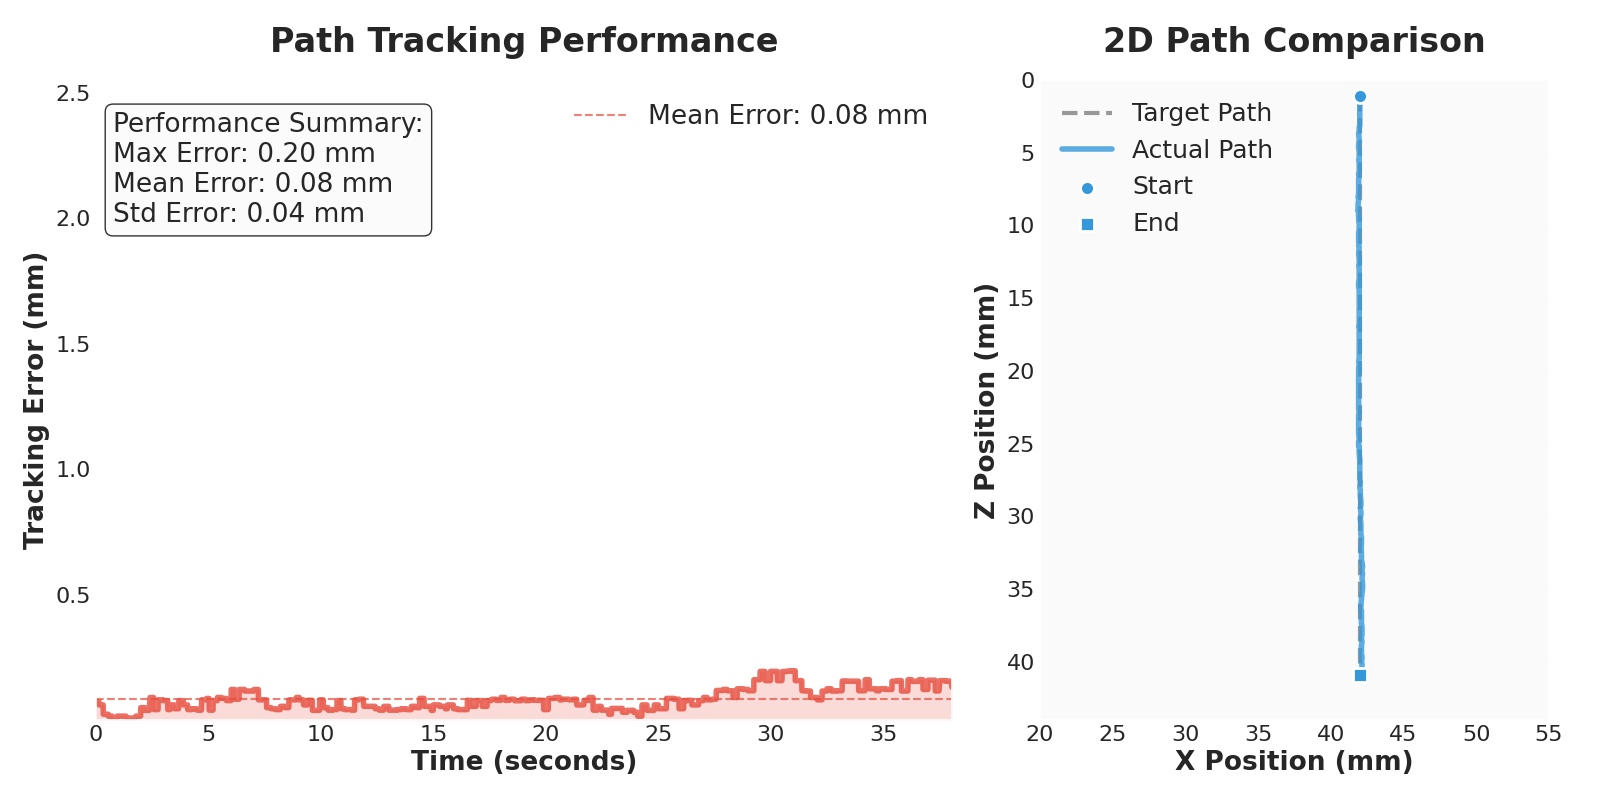
\includegraphics[width=\linewidth]{images/pathfollowing/ILOS/straight_250704_164227_scaled.png}
    \caption{Straight line ILOS path following performance in a brain phantom}
    \label{fig:straightILOS}
\end{figure}


\subsubsection{Path 1: Comparing Open-Loop and Closed-Loop}
To evaluate the performance of open-loop versus closed-loop control on a more complex trajectory, where the open-loop applies not just neutral tension but the same feedforward tensions used in the closed-loop case, both systems were tested on a curved path through the brain phantom. This path has straight segments as well as two different curvature segments, making it a lot more challenging than the straight-line scenario.

\paragraph*{Open-Loop Path-Following}

As shown in figure \ref{fig:curvedol}, the open-loop guidance system performs poorly when following the curved path. Although the system applies different tensions for every segment that corresponds to the actuation values determined appropriate for those curvature, it reults in a steadily increasing deviation from the target trajectory. There is significant drift leading to a maximum tracking error of 9.44mm, and a mean error of 3.48mm. 
\begin{figure} [H]
    \centering
    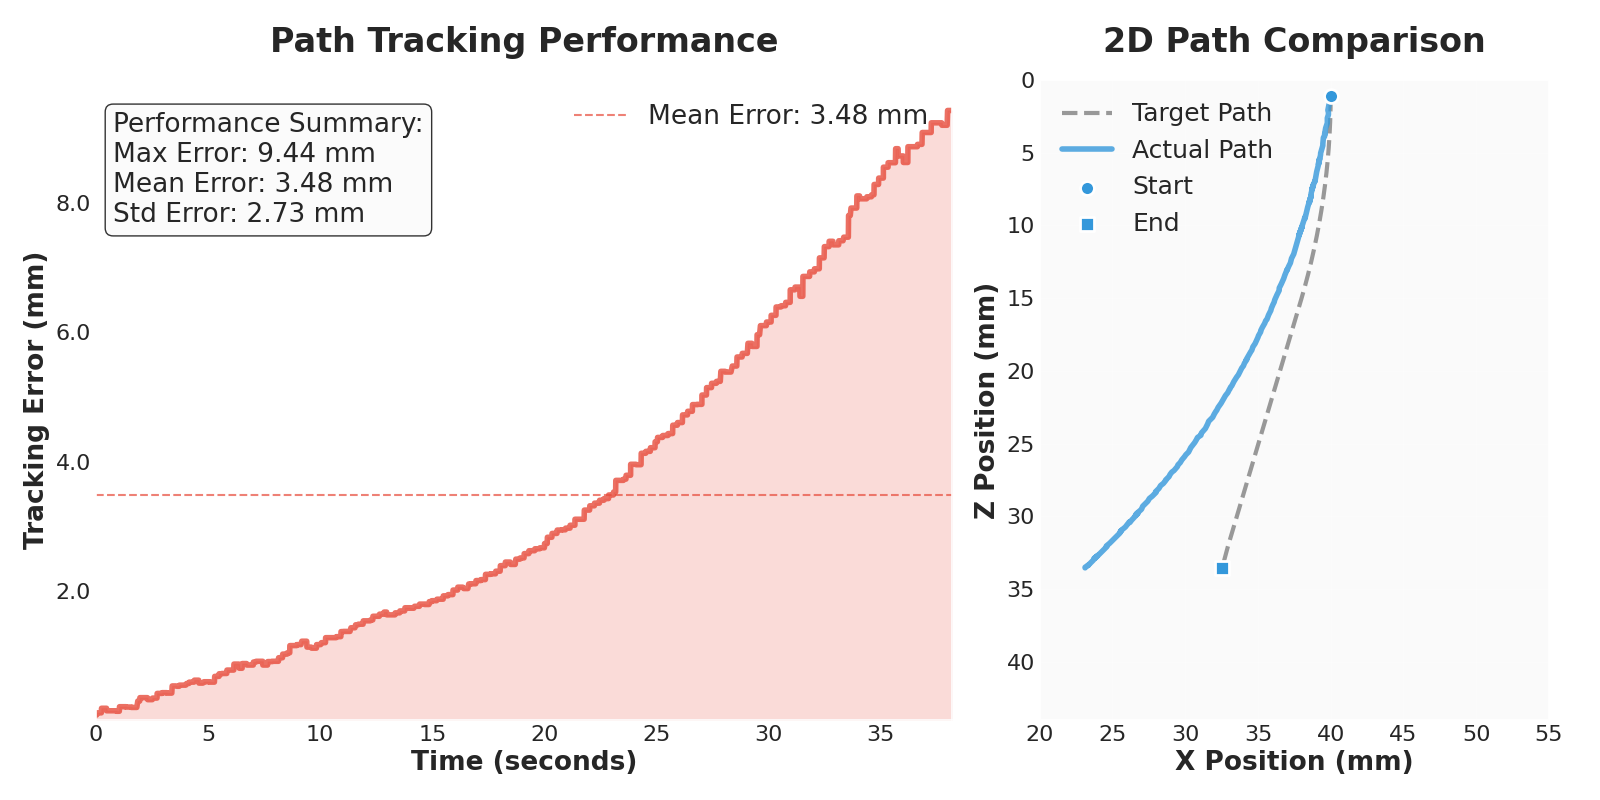
\includegraphics[width=\linewidth]{images/pathfollowing/openloop/longleft_250703_120246.png}
    \caption{Open-Loop path-following performance on a curved trajectory in the brain phantom}
    \label{fig:curvedol}
\end{figure}


\paragraph*{Closed-Loop (LOS) Path-Following}

\begin{figure} [H]
    \centering
    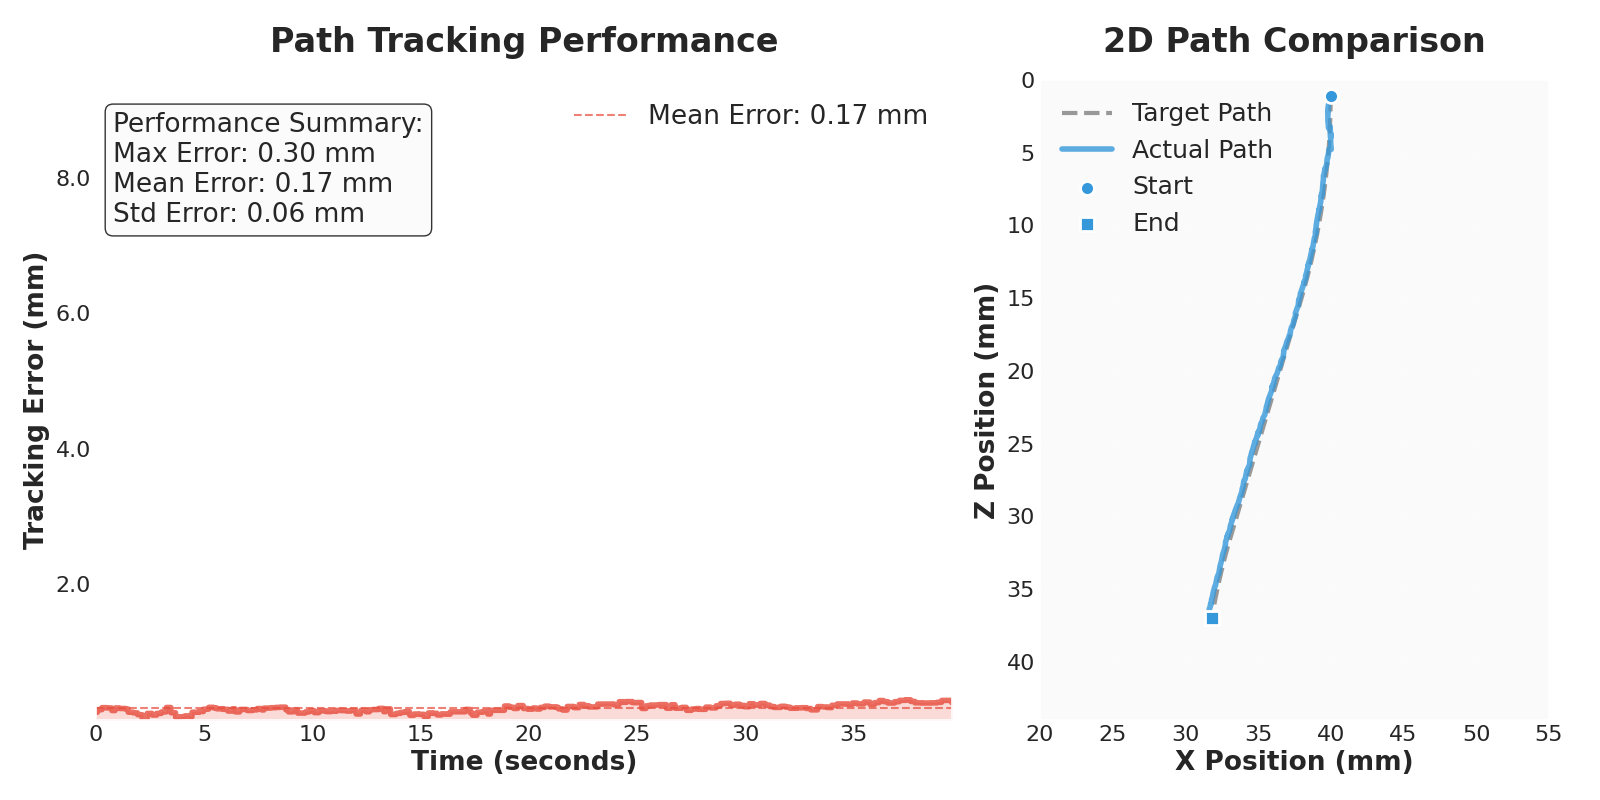
\includegraphics[width=\linewidth]{images/pathfollowing/LOS/longleft_250703_115622_scaled.png}
    \caption{Closed-Loop (LOS) path-following performance on a curved trajectory in the brain phantom}
    \label{fig:curvedcl}
\end{figure}
Figure \ref{fig:curvedcl} shows the effectiveness of the closed-loop LOS controller on the same curved path. The mean error is reduced to 0.17mm, and the maximum error to 0.3mm, a decrease of 9.14mm. 

\subsubsection{Path 2: Comparing LOS and ILOS}
In order to test the difference between the LOS and ILOS guidance systems, both were tested on the same two-curvature path. Because the ILOS system is expected to minimize steady state error both ribbons were intentionally started a small distance (0.4mm) away from the starting point of the target path to challenge the two systems ability to correct this initial offset. 
\subsubsection{LOS Path-Following}
\begin{figure} [H]
    \centering
    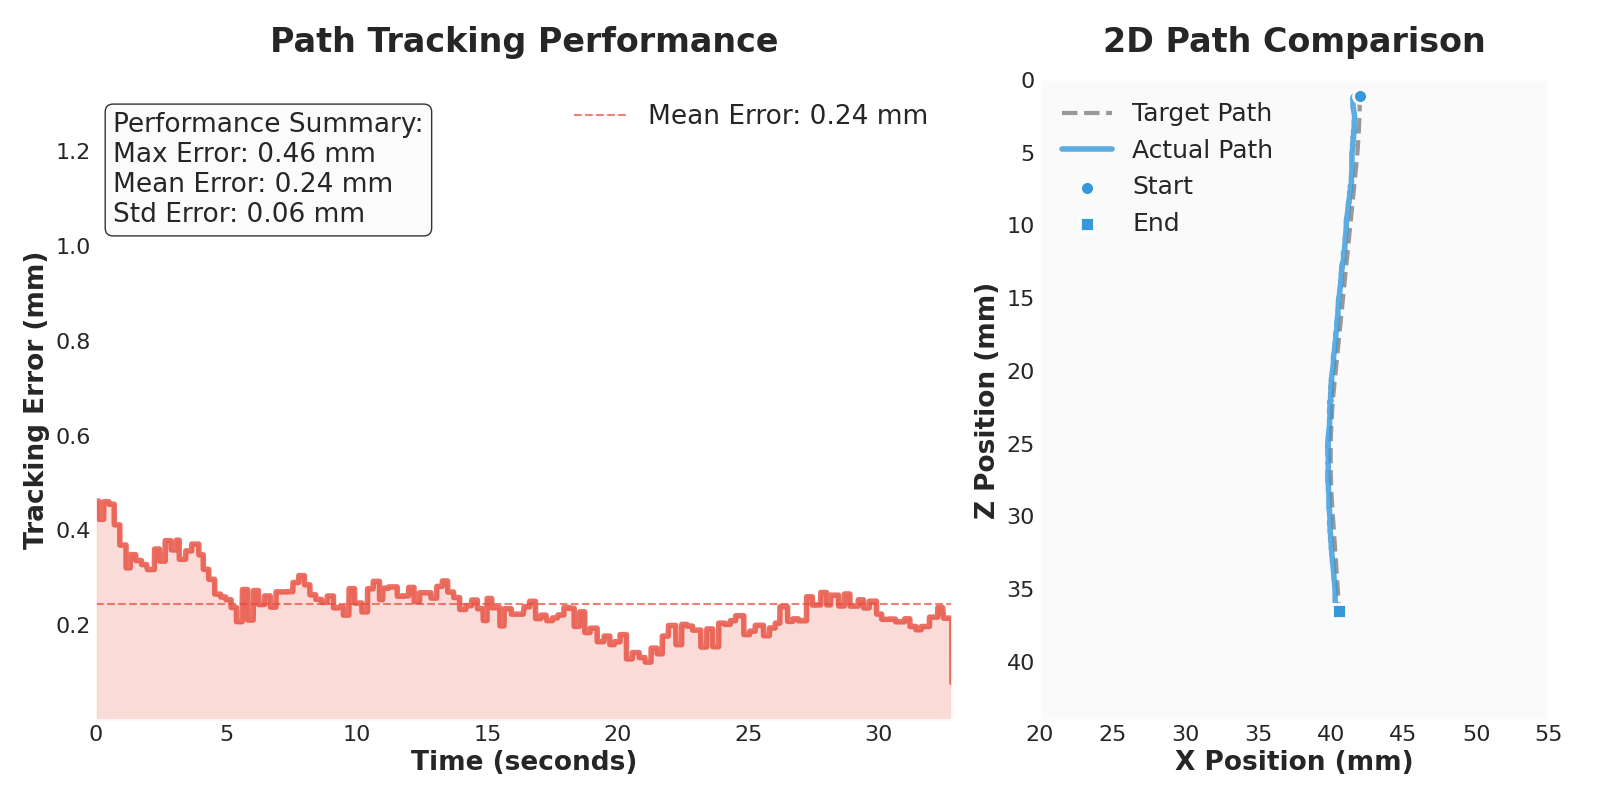
\includegraphics[width=\linewidth]{images/pathfollowing/LOS/twocurves_250704_151624.png}
    \caption{LOS path-following performance on a curved path with a small starting offset}
    \label{fig:LOStwocurves}
\end{figure}
As shown in figure \ref{fig:LOStwocurves}, the LOS controller achieves a tracking with a mean error of 0.24mm. However largely due to the initial starting offset of approximately 0.4mm, there is a noticeable steady-state error of around 0.2mm  that remains throughout the trial. 

\paragraph*{ILOS Path-Following}
\begin{figure} [H]
    \centering
    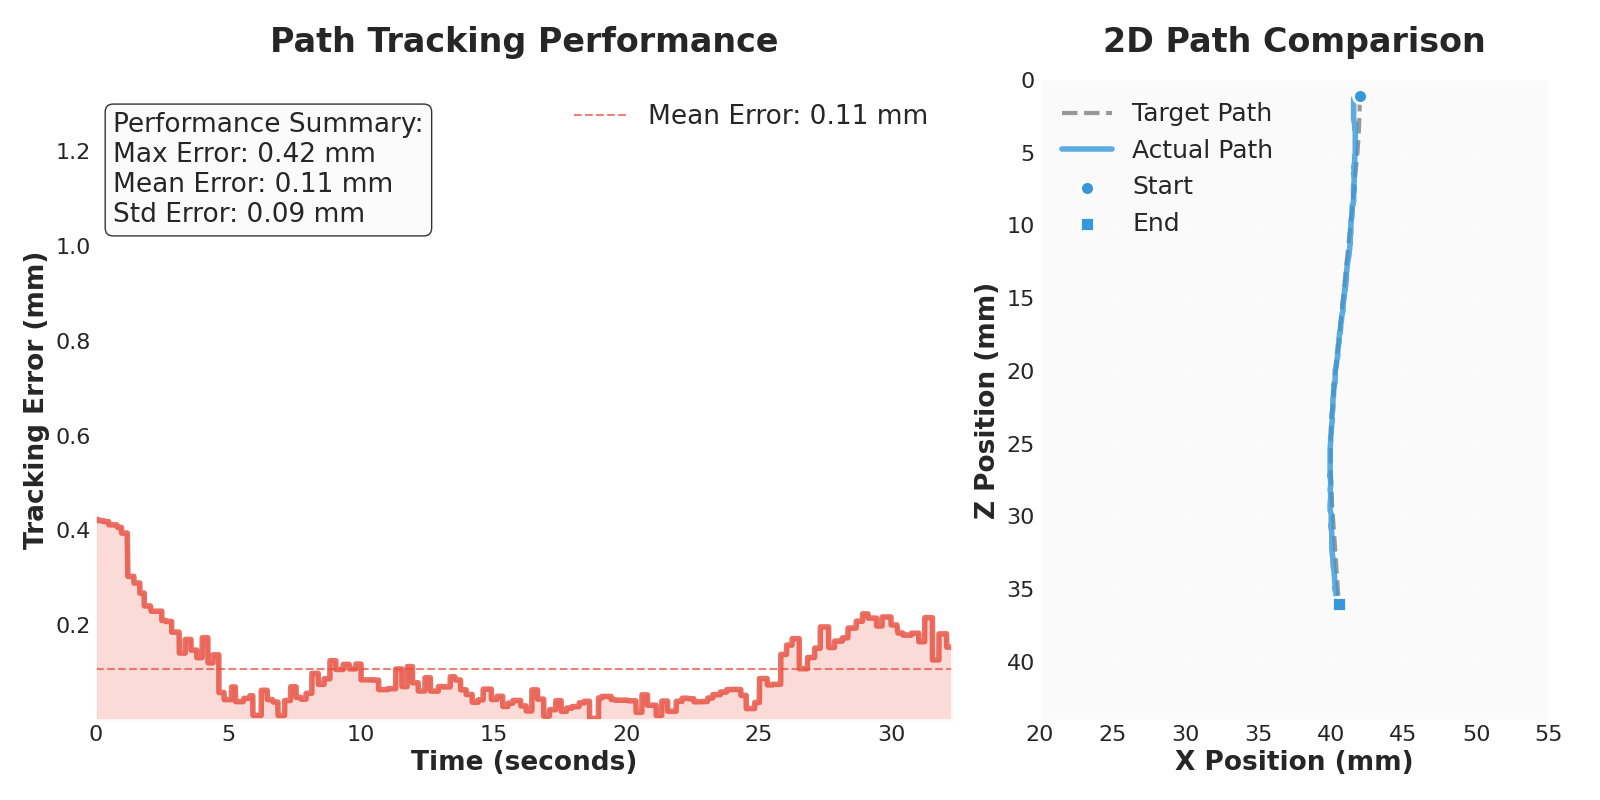
\includegraphics[width=\linewidth]{images/pathfollowing/ILOS/twocurves_250704_153907_2K5i.png}
    \caption{ILOS path-following performance on a curved path with a small starting offset}
    \label{fig:ILOStwocurves}
\end{figure}
Figure \ref{fig:ILOStwocurves} shows that the ILOS guidance system performs with higher precision and better convergence. The mean error is reduced to 0.11mm mostly due to the systems ability to eliminate the the steady-state error visible in the LOS system. The 2D path comparison shows a nearly perfect alignment between the actual and target paths after an initial period of convergence because of the initial offset.




\subsection{Discussion}

\subsubsection{Ribbon Adaptation}
While the ribbon adaption method significantly improves performance, it does not perfectly capture the ribbon's true behavior. First, the characterization is done in air (for the reasons outlined in the design section). Second, the ribbon has a very distinct hysteresis effect that is not explicitly modeled. The hysteresis loop shows that the dynamics cannot in reality be modeled using a single-valued function. Although the fitted model still uses a simplified three-segment piecewise function, the actual system depends on the history of previous states. This has implications for control accuracy, particularly during rapid or alternating actuation cycles.
\newline \newline
This imperfect adaptation also leads to the need for slight adjustments to the PI gains (for optimal performance) for the right and left pitch feedback control to adapt it to the ribbon. Before implementing the ribbon adaptation module, this tuning process was very time-consuming and absolutely essential for acceptable performance. With the adaptation module, one can achieve acceptable performance without re-doing the tuning, but tweaking for each ribbon will lead to better performance. The results presented above were obtained after making minor adjustments to the default PI values to tailor to that ribbon. Ideally, such manual tuning would be unnecessary if the ribbon dynamics were more consistent or if the ribbon adaptation method fully captured all relevant behaviors.
\newline \newline 
Additionally the observations made with regards to the affects of water and gelatin also suggests that tendon lubrication is essential. Without it, friction within the tendon channels likely prevents smooth tendon motion, resulting in impaired bending. As a result, it should be standard practice to dip the ribbon in water before each calibration or experiment.

\subsubsection{Open-Loop Performance}
The results for straight path following show that the open-loop system performs poorly, as expected. Without feedback, the inherent pre-curvature of each ribbon causes significant drift,. This is because small deviations in expected tip curvature accumulate over the insertion distance in gelatin leading to large errors in position
\newline \newline
Similarly, for curved paths, the open-loop system applies feedforward actuation values determined during charactarization on a different ribbon. Since each ribbon's dynamics differ significantly this likely led to the poor performance seen in figure \ref{fig:curvedol}. These results clearly demonstrate that feedback is essential, even when thorough characterization has been performed.

\subsubsection{LOS Performance}
The LOS guidance system is, from the results, a huge improvement over open-loop control, reducing drift and maintaining stable, low tracking errors (<0.4mm) in both straight and curved paths. This also validates the modeling the ribbon's behavior to be similar to that of vessel. It is also worth noting that the path seen in figure \ref{fig:curvedcl} pushes the limits of what that ribbon is capable of according to its dynamics identified in air. This path includes segments that have curvatures which are the  maximum curvatures that this ribbon can achieve in air, making such accurate tracking especially impressive.
\newline \newline
However LOS exhibits small steady-state offsets, particularly when starting from a misaligned position as in \ref{fig:LOStwocurves}. This can be partly attributed to variations in the mechanical properties of the gelatin phantom, and unmodeled kinematic attributes of the ribbon such as its hysteresis. If the medium is stiffer than expected or the tendon actuation does not produce the anticipated tip curvature, small deviations can accumulate into steady-state errors that traditional LOS cannot fully correct. This is  analogous to how a boat following a planned course with LOS will experience a steady-state error if subjected to unexpected current, since LOS cannot correct for such external factors. This was however an expected result and was why ILOS was hypothesized to be a better alternative for the system.

\subsubsection{Final (ILOS) Path-Following Performance}
The use of ILOS guidance for this application is as far as the author knows is the first use of this type of guidance system for a continuous device and therefore represents a novel approach to path following. While ILOS is typically applied in marine and aerial robotics to compensate for environmental disturbances, its adaptation here to navigation in soft brain-like tissue in order to compensate for modeling inaccuracies and varying stiffness's is clearly a successful approach. And one it could expect it to be even more important to have the integral term in a more heterogeneous medium than the brain phantom used here, such as the real brain.
\newline \newline
The ILOS controller outperforms the traditional LOS with tracking errors reamining consistently below 0.15mm, even in curved trajectories and with intentional initial offsets. The system integral term is clearly successfull in eliminating the small steady-state errors observed with LOS. 

\subsubsection{Final Performance Compared to Other Neurosurgical Methods}
The ILOS straight line performance of 0.08mm \(\pm \) 0.04mm error and 0.08mm \(\pm\) 0.06mm error during curved line following (after compensating for the inital intentional offset) is an extremely high level of accuracy. Comparing with the state of the art closed-loop methods duty cycle needle steering was reported to have an accuracy of 0.71mm when simulated in a kidney phantom \cite{wood_needle_2010}, this was notably however using much more lenient curvatures (max 0.003mm\(^{-1}\)) \cite{wood_needle_2010} compared to the path tested here (0.022mm\(^{-1}\)). An even closer comparison would be to that of closed-loop control of programmable bevel-tip needle in a gelatin brain phantom, where the accuracy is reported to be 0.68mm \(\pm\)1.45mm, with again much smaller curvatures of 0.0056mm\(^{-1}\) \cite{ko_closed-loop_2011}, thus the accuracy of the ILOS system is roughly an order of magnitude better than these methods. 
\begin{figure}[H]
    \centering
    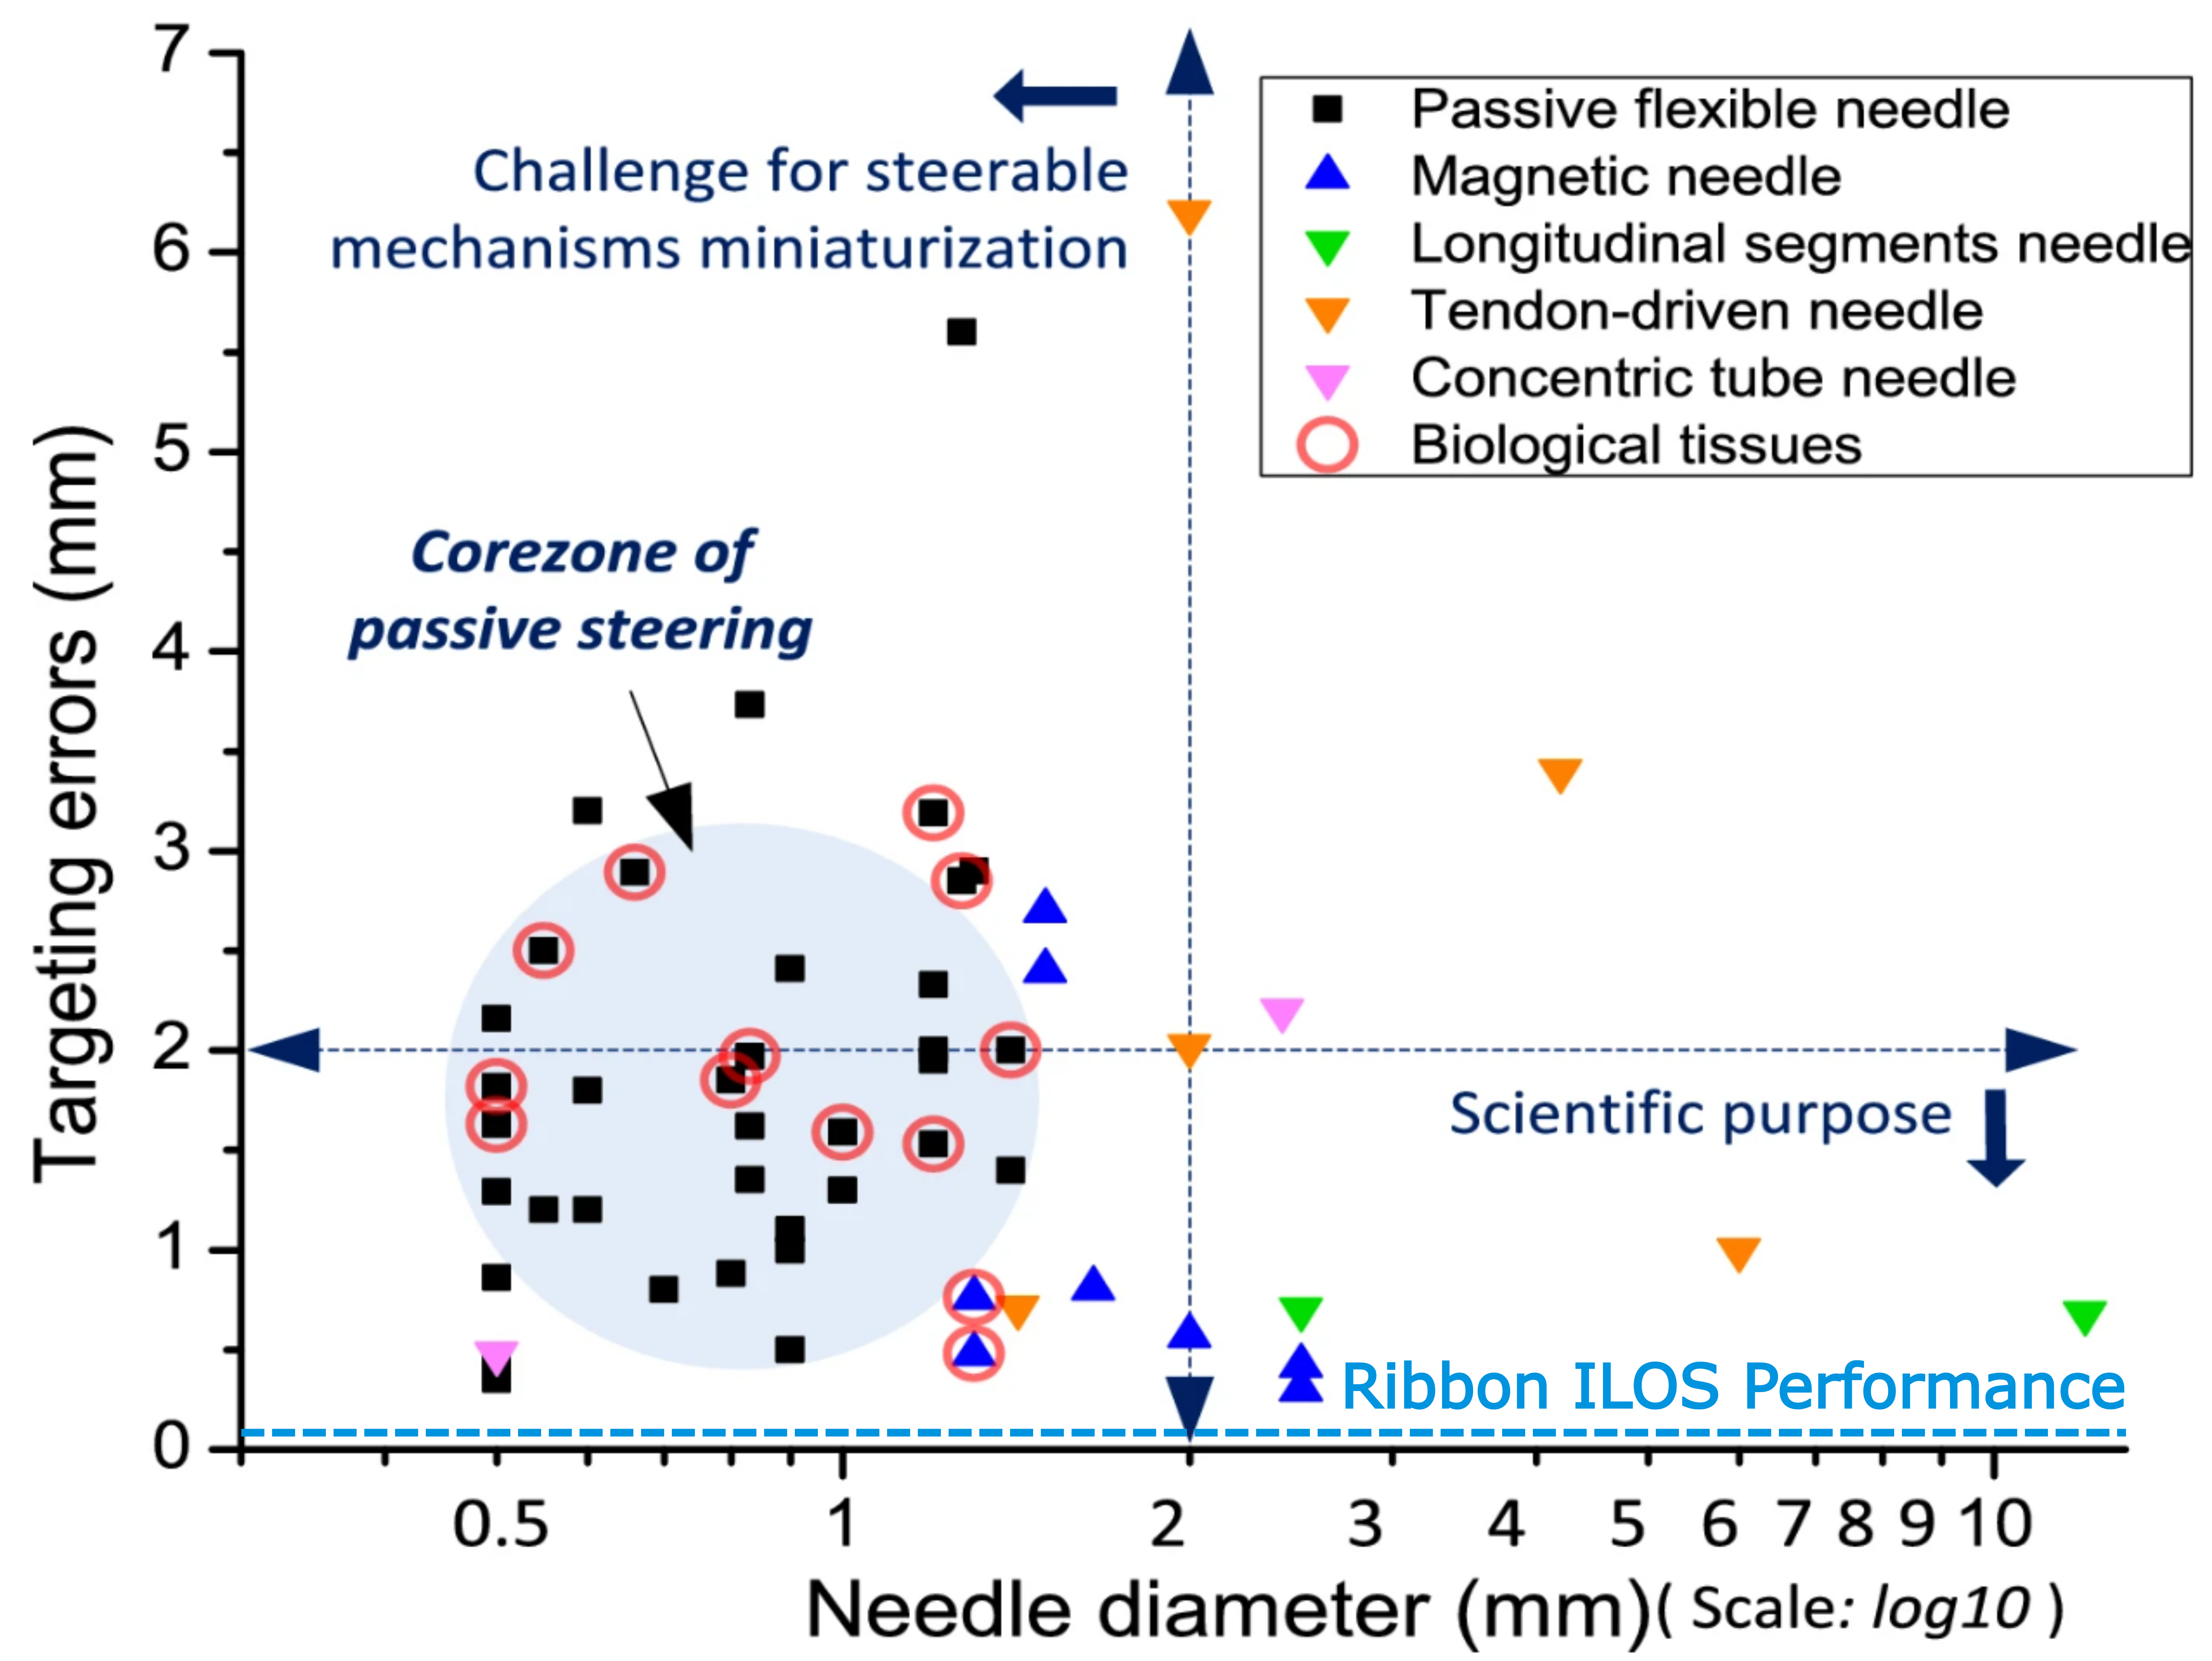
\includegraphics[width=0.95\linewidth]{images/pathfollowing/performanceCompared4.png}
    \caption{Figure adapted from \cite{lu_flexible_2023} showing the performance of current studies of flexible needle steering, compared to the performance of this system using ILOS}
    \label{fig:performanceCompared}
\end{figure}
According to a review on flexible needles published in 2023 which surveys 131 articles \cite{lu_flexible_2023}.For a comparison of the Ribbon ILOS performance and all reported steerable needle performance see figure \ref{fig:performanceCompared}. The best reported performance in that review is that of a magnetically steered needle that acheives a 0.3mm accuracy in a brain phantom \cite{hong_magnetic_2021}.  A very low error, but also over three times that of this system, proving the effectiveness of the novel ILOS-based approach which also has the benefit of necessitating much less exact modeling compared to these other systems. 
\newline \newline
In a clinical context, stereotactic neurosurgical guidance systems, such as those used for deep brain stimulation electrode placement, typically report targeting accuracies between 0.6mm and 1.3mm \cite{zacest_precision_2009}, \cite{rajabian_accuracy_2022}, \cite{moser_measurement_2012}. However 2-3mm errors are tolerated by most surgical needle placement procedures, and manual placement error is approximately 3-5mm \cite{rucker_sliding_2013}. Frame-based stereotaxy remains the gold standard with sub millimeter accuracy reported but rarely below 0.3-0.5mm in practice \cite{roth_accuracy_2018}.
\newline \newline
Although testing remains to be done in vitro, and more thorough randomized testing should be done in gelatin the 0.08mm accuracy strongly suggests that the ILOS closed-loop design and ribbon device have the potential to not only surpass the current state-of-the-art in needle steering, but also to outperform manual methods and possibly approach or exceed the gold standard of frame-based stereotaxy in clinical accuracy.





\subsection{Future Development}

\subsubsection{Further Ribbon Adaptation}
One of the main areas for future work is the ribbon adaptation method, this could be changed so that instead of only identifying which tendon actuation should be applied based on the desired curvature, it should also be based on the history, the previous states. This way it could take into account the very pronounced hysteresis effect of the ribbon. Thorough mappings between how the curvature profiles look in air vs gelatin should also be made in order to further validate the current adaptation process.
\newline \newline
Another possible avenue for exploration is online adaptation. For example using online model-performance optimization using extremum seeking to tune thi PI gains of the pitch converter \cite{killingsworth_pid_2006}. This would improve the performance without manual retuning and remove the need for an axect ribbon adaptation module.

\subsubsection{Future Hardware Iterations}
The main limitation of the current system stem from the ribbon devices themselves. The manufacturing leads to inconsistent dynamics between devices. Additionally interaction with gelatin and dust cause further unpredictable changes in curvature performance. A recurring issue has also been tendon breakage. However this was significantly improved by regular cleaning and ripping the ribbon in water prior to actuation.
\newline \newline 
Achieveing robust control remains challenging due to the variation in dynamics. Therefore future work should aim improving the consistency and durability of the ribbon devices. Currently there is already a project underway to miniaturize the device, further expanding its potential.

\subsubsection{Extension to 3D PathFollowing}
A final major avenue for future work is the extension to 3D path following. Due to time constraints and the unexpectedly broad scope of tasks during this thesis, it was decided that achieving robust 2D control should be prioritized over attempting a 3D implementation. However, the ribbon’s capability for both twisting and bending maneuvers makes 3D control a natural next step.
\newline \newline
One approach is to draw inspiration from fixed-wing aircraft control or bank-to-turn strategies. Since the ribbon cannot simultaneously twist and bend, a control strategy could involve incorporating twisting into the planned path. A dedicated ILOS-based controller could be used to track the ribbon's twist angle, reorienting the bending plane to ensure that the path points lie withing the reachable 2D plane. Once the plane is aligned through twisting, a separate ILOS controller, the 2D controller developed for this thesis can handle the bending control withing that plane to follow the desired path. Since bending and twisting will not happen simultaneously one could switch between these modes control based on the pre-planned path and the observed errors. This staged control, alternating between twisiting and bending and combining it with ILOS may offer a promising path toward full 3D trajectory following.




